\documentclass[a4paper]{article}
\usepackage{geometry}
\geometry{
	a4paper,
	total={170mm,257mm},
	left=27mm,
	right=30mm,
	top=30mm,
	bottom= 30mm
}
\usepackage{tabu}
\usepackage[english]{babel}
\usepackage[utf8]{inputenc}
\usepackage{longtable}
\usepackage{amsmath}
\usepackage{graphicx}
\usepackage{enumitem}
\usepackage[colorinlistoftodos]{todonotes}
\usepackage{tikz}
\newcommand*\circled[1]{\tikz[baseline=(char.base)]{
		\node[shape=circle,draw,inner sep=0.5pt] (char) {#1};}}
\usetikzlibrary{fit,positioning}
\usepackage{authblk}
\usepackage{natbib}
\usepackage[algo2e]{algorithm2e}
\usepackage{algorithmic}  
\usepackage{algorithm}
\usepackage{comment}
\usepackage{array}% http://ctan.org/pkg/array
\makeatletter
\g@addto@macro{\endtabular}{\rowfont{}}% Clear row font
\makeatother
\newcommand{\rowfonttype}{}% Current row font
\newcommand{\rowfont}[1]{% Set current row font
	\gdef\rowfonttype{#1}#1%
}
\newcolumntype{L}{>{\rowfonttype}l}
\title{A Network Model for Dynamic Textual Communications \\with Application to
	Government Email Corpora}
%\author{Bomin Kim}

\author[1]{Bomin Kim}
\author[1]{Zachary Jones}
\author[1]{Bruce Desmarais}
\author[2,3]{Hanna Wallach}
\affil[1]{Pennsylvania State University}
\affil[2]{Microsoft Research NYC}
\affil[3]{University of Massachusetts Amherst}

\begin{document}
\maketitle
\begin{abstract}
	
	\noindent In this paper, we introduce the interaction-partitioned topic model
	(IPTM)---a probabilistic model of who communicates with whom about
	what, and when. Broadly speaking, the IPTM partitions time-stamped
	textual communications, such as emails, according to both the network
	dynamics that they reflect and their content. To define the IPTM, we
	integrate a dynamic version of the exponential random graph model---a
	generative model for ties that tend toward structural features such as
	triangles---and latent Dirichlet allocation---a generative model for
	topic-based content. The IPTM assigns each topic to an "interaction
	pattern"---a generative process for ties that is governed by a set of
	dynamic network features. Each communication is then modeled as a
	mixture of topics and their corresponding interaction patterns. We use
	the IPTM to analyze emails sent between department managers in two
	county governments in North Carolina; one of these email corpora
	covers the Outer Banks during the time period surrounding Hurricane
	Sandy. Via this application, we demonstrate that the IPTM is effective
	at predicting and explaining continuous-time textual communications.
\end{abstract}
\section{Introduction} \label{sec: Introduction}

In recent decades, real-time digitized textual communication has developed into a ubiquitous form of social and professional interaction \citep[see, e.g.,][]{kanungo2008modeling, szostek2011dealing, burgess2004email, pew2016}. From the perspective of the computational social scientist, this has lead to a growing need for methods of modeling networks consisting of text-valued edges that arise in continuous time (e.g., e-mail messages). A number of models that build upon topic modeling through Latent Dirichlet Allocation \citep{Blei2003} to incorporate link data as well as textual content have been developed in response to this need {\bf [ASK HANNA FOR CITES]}.  The exponential random graph model (ERGM) \citep{robins2007introduction,chatterjee2013estimating,hunter2008ergm}, which is the canonical model for network structure as it is flexible enough to account for nearly any pattern of tie formation \citep{desmarais2017statistical}, has yet to be adapted to the setting of time-stamped text-valued edges. We build upon recent extensions of ERGM that model time-stamped ties \citep{PerryWolfe2012,Butts2008}, and develop the interaction-partitioned topic model (IPTM) to simultaneously model the network structural patterns that govern tie formation, and the content in the communications.\\ \newline
In defining and testing the IPTM we embed three core conceptual properties, in addition to modeling both text and network structure. First, we link the content component of the model, and network component of the model such that knowing who is communicating with whom at what time (i.e., the network component) provides information about the content of communication (i.e., the content component),  and vice versa. Second, we fully specify the network dynamic component of the model such that, given the content of the communication and the history of tie formation, we can draw an exact, continuous-time prediction of when and to whom the communication will be sent. Third, we formulate the network dynamic component of the model such that the model can represent, and be used to test hypotheses regarding, canonical processes relevant to network theory such as preferential attachment {\bf [popularity cites]}, reciprocity {\bf [reciprocity cites]}, and transitivity {\bf [transitivity cites]}. In what follows we (1) present the generative process for the IPTM, describing how it meets our theoretical criteria, (2) derive the sampling equations for Bayesian inference with the IPTM, and (3) illustrate the IPTM through application to email corpora of internal communications by county officials in North Carolina county governments. {\bf [What predictive comparisons should we run to other models]}?

\begin{comment}
Since Latent Dirichlet Allocation \citep{Blei2003}, which models of words alone, a variety of useful topic models have been developed by considering additional components other than words. One direction incorporated the network aspect by using the author and receiver information such as Author-Topic Models \citep{rosen2004author}, Author-Recipient-Topic Models and Role-Author-Recipient-Topic Models \citep{mccallum2005topic}, however, all of the models treat the author and recipients as observed variable thus generative processes only involve topics and words in a document. On the other side, there have been a lot of topic
models that focus on the timestamps of documents. For example, Dynamic Topic Models \citep{blei2006dynamic} introduced logistic normal topic models that rely on Markov assumptions with discretization of time, and Topics Over Time \citep{wang2006topics} suggested a countinuous-time model by generating a timestamp from the Beta distribution with its parameter depending on each topic assignment. However none of the above mentioned topic models are jointly dealing with the author-recipient and timestamps of the documents, although it is common in the field of dynamic network analysis to study who connects to whom and when $(i, j, t)$. 
\end{comment}

\section{Generative Process} \label{sec: Generative Process}
Assume we have a collection of documents, consisting of $D$ number of unique documents. A single email, indexed by $d \in \{1,...,D\}$, is represented by the four components ($i^{(d)}, J^{(d)}, t^{(d)},  \boldsymbol{w}^{(d)}$). The first two are the sender and receiver of the email: an integer $i^{(d)} \in \{1,...,A\}$ indicates the identity of the sender out of $A$ number of actors (or nodes) and an integer vector $J^{(d)} = \{j_r^{(d)}\}_{r=1}^{|J^{(d)}|} $ indicates the identity of the receiver (or receivers) out of $A-1$ number of actors (by excluding self-loop), where $|J^{(d)}|\in \{1,...,A-1\}$ denotes the total number of the receivers. Next, $t^{(d)}$ is the (unix time-based) timestamp of the email $d$, and $\boldsymbol{w}^{(d)} = \{w^{(d)}_m \}_{n=1}^{N^{(d)}}$ is a set of tokens that comprise the text of the email. In this section, we illustrate how the words $\boldsymbol{w}^{(d)}$ are generated according to the variant of latent Dirichlet allocation \citep{Blei2003}, and then how the rest three components, ($i^{(d)}, J^{(d)}, t^{(d)}$), are simulatneously generated from the stochastic intensity and topic assignments of the document. For simplicity, we assume that documents are ordered by time such that $t^{(d)} < t^{(d+1)}$ for all $d=1, ..., D$.
\subsection{Content Generating Process} \label{subsec: Content Generating Process}
The content generating process is a simple addition of the interaction pattern assignment to the existing generative process of Latent Dirichlet Allocation \cite{Blei2003}. This concept is also very similar to the content-partitioned multinetwork embeddings (CPME) model {\bf [ASK BRUCE FOR CITES]}, in a way that each topic $k$ is also associated with a cluster assignment $c_k$, where $c_k$ can take one of $c = \{1,...,C\}$ values. \\ \newline
First we generate the global (corpus-wide) variables. There are two main sets of global variables:
those that describe the topics people talk about and those that describe how people interact (interaction patterns). These variables are linked by a third set of variables that associate each topic with the pattern that best describes how people interact when talking about that topic.\\ \newline
There are $K$ topics. Each topic $k$ is a discrete distribution over $V$ word types.
\begin{itemize}
	\item[1.] {$\boldsymbol{\phi}^{(k)} \sim \mbox{Dir}(\beta, \bf u)$} \textbf{[See Algorithm 1]}\\
	- A “topic” $k$ is characterized by a discrete distribution over $V$ word types with probability vector $\phi^{(k)}$. A symmetric Dirichlet prior $\bf u$ with the concentration parameter $\beta$ is placed.
\end{itemize}
\noindent There are $C$ interaction patterns. Each interaction pattern consists of a vector of coefficients $\boldsymbol{b}^{(c)}$ in $\boldsymbol{R}^{P}$ and a vector of P-dimensional dynamic network statistics for directed edge $(i, j)$ at time $t$ $\boldsymbol{x}^{(c)}_t(i, j)$; however, we assume that our generative process is conditioned on these covariates. 
\begin{itemize}
	\item[2.] $\boldsymbol{b}^{(c)}\sim \mbox{Normal}(\textbf{0}, \sigma^2I_P)$ \textbf{[See Algorithm 2]}: \\
		- The vector of coefficients depends on the interaction pattern $c$. This means that there is variation in the degree of influence from the dynamic network statistics.
	\end{itemize}
\noindent The topics and interaction patterns are tied together via a set of $K$ categorical variables.
\begin{itemize}
	\item[3.] $c_k\sim \mbox{Unif}(1, C)$ \textbf{[See Algorithm 3]}: \\
	- Each topic is associated with a single interaction pattern.\\
\end{itemize}
\noindent Then, we generate the local variables. We assume the following generative process for each document $d$ in a corpus $D$ \textbf{[See Algorithm 4]}:
\begin{itemize}
	\item[4-1.] Choose the number of words $N^{(d)} = \mbox{max}(1, \bar N^{(d)})$, where $\bar N^{(d)}\sim \mbox{Poisson}(\zeta)$
	\item[4-2.] Choose document-topic distribution $\boldsymbol{\theta}^{(d)}\sim \mbox{Dir}(\alpha, \boldsymbol{m})$
	\item[4-3.] For $n=1$ to $N^{(d)}$:
	\begin{itemize}
		\item[(a)] Choose a topic $z_n^{(d)} \sim \mbox{Multinomial}(\boldsymbol{\theta}^{(d)})$
		\item[(b)] if $\bar N^{(d)}>0$, choose a word $w_n^{(d)} \sim\mbox{Multinomial} (\phi^{(z_n^{(d)})})$
	\end{itemize}
\end{itemize}
\subsection{Stochastic Intensity} \label{subsec: Stochastic Intensity}
Here we illustrate how a set of dynamic network features and topic-interaction assignments  jointly identify the stochastic intensity of a document, which plays a key role in tie generating process in \ref{subsec: Tie Generating Process}. Assume that each document $d \in \{1,...,D\}$ has an $A\times A$ stochastic intensity (or hazard) matrix of $\boldsymbol{\lambda}^{(d)}(t) = \{\{\lambda^{(d)}_{ij}(t)\}_{i=1}^{A}\}_{j=1}^{A}$, where $\lambda^{(d)}_{ij}(t)$=P\{for document $d$, $i\rightarrow j$ occurs in time interval $[t, t+dt)$, given that it has not ben sent until time $t$\}. \\ \newline
To calculate the distribution of interaction patterns within a document, we estimate the (empirical) proportion of the words in document $d$ which are assigned the topics corresponding to the interaction pattern $c$ from \ref{subsec: Content Generating Process}: 
\begin{equation}
p_c^{(d)} = \frac{\sum\limits_{k: c_k=c} N^{(k|d)}}{N^{(d)}},
\end{equation}
where $N^{(k|d)}$ is the number of times topic $k$ shows up in the document $d$, and $\sum\limits_{c=1}^{C}p_c^{(d)}=1$.\\\\ \newline
Now, we define the $(i, j)^{th}$ element of the stochastic intensity matrix $\boldsymbol{\lambda}^{(d)}(t)$ forms:
\begin{equation}
\lambda^{(d)}_{ij}(t)=\sum\limits_{c=1}^{C} p^{(d)}_c
\cdot  \mbox{exp}\Big\{\lambda^{(c)}_0\cdot \boldsymbol{b}^{(c)T}\boldsymbol{x}^{*(c)}_t(i, j)\Big\}\cdot 1\{j \in \mathcal{A}_{\backslash i}\},
\end{equation}
where $p_c^{(d)}$ is as defined above, $\lambda^{(c)}_0$ is the baseline hazards for the interaction pattern $c$, $\boldsymbol{b}^{(c)}$ is an unknown vector of coefficients in $\boldsymbol{R}^{p}$ corresponding to the interaction pattern $c$, $\boldsymbol{x}^{*(c)}_t(i, j)$ is a vector of the $p$-dimensional dynamic network statistics for directed edge $(i, j)$ at time $t$ corresponding to the interaction pattern $c$, and $\mathcal{A}_{\backslash i}$ is the predictable receiver set of sender $i$ within the set of all possible actors $\mathcal{A}$ (no self-loop). After we include intercept and set $\boldsymbol{x}^{(c)}_t(i, j)=(\boldsymbol{1}, \boldsymbol{x}^{*(c)}_t(i, j))$, we rewrite (2) as: 
\begin{equation}
\lambda^{(d)}_{ij}(t)= \sum\limits_{c=1}^{C} p^{(d)}_c\cdot\mbox{exp}\Big\{\boldsymbol{b}^{(c)T}\boldsymbol{x}^{(c)}_t(i, j)\Big\}\cdot 1\{j \in \mathcal{A}_{\backslash i}\},
\end{equation}
where now the first element of $\boldsymbol{b}^{(c)}$ corresponds to the baseline intensity of interaction pattern $c$. This $\lambda$ can be seen as the weighted average of stochastic intensities across the interaction patterns. Next, since multicast interactions—those involving a single sender but multiple
receivers—are allowed for this model, we expand the rate of interaction between sender $i$ and the receivers in a set $J$ by taking the average of $\boldsymbol{b}^{(c)T}\boldsymbol{x}^{(c)}_t(i, j)$ terms across the receivers:
\begin{equation}
\lambda^{(d)}_{iJ}(t)= \sum\limits_{c=1}^{C} p^{(d)}_c\cdot\mbox{exp}\Big\{\frac{1}{|J|}\sum\limits_{j \in J} \boldsymbol{b}^{(c)T}\boldsymbol{x}^{(c)}_t(i, j)\Big\}\cdot \prod\limits_{j \in J}1\{j \in \mathcal{A}_{\backslash i}\}.
\end{equation}
In case of single receivers ($|J|=1$),  Equation (4) is reduced to Equation (3), thus in the following sections we use the Equation (4) of multicast cases as a general form of the stochastic intensity between the sender and receivers.
\begin{comment}
Conditioned upon the existence of a unique document at some particular time $t$, the probability that the document is sent from $i$ to $j$ is
	\begin{align*}
	&L_{ij}(\boldsymbol{b}^{(c)}) = \frac{\mbox{exp}\Big\{ \boldsymbol{b}^{(c)T}\boldsymbol{x}^{*(c)}_t(i, j)\Big\}}{\mbox{exp}\Big\{\sum\limits_{j \in \mathcal{A}_{\backslash i}} \boldsymbol{b}^{(c)T}\boldsymbol{x}^{*(c)}_t(i, j)\Big\}},
	\end{align*}
and considering the multicasts and treating the documents being statistically independent, the joint probability, the full likelihood function is:
\begin{equation}
L(\boldsymbol{b}^{(c)})=\prod_{d: c^{(d)}=c} \frac{\mbox{exp}\{\sum\limits_{j \in J^{(d)}} \boldsymbol{b}^{(c)T}x^{(c)}_{t^{(d)}}(i^{(d)}, j)\}}{\sum\limits_{\substack{J \subseteq \mathcal{A}_{\backslash i^{(d)}} \\|J|=|J^{(d)}|}} \mbox{exp}\{\sum\limits_{j \in J} \boldsymbol{b}^{(c)T}x^{(c)}_{t^{(d)}}(i^{(d)}, j)\}}.
\end{equation}
This is exactly the form of the partial likelihood function of \cite{cox1992regression}, however, in our case it is full likelihood since we do not have baseline hazard (incorporated into $\boldsymbol{x}$) in $\lambda^{(c)}_{ij}(t|\boldsymbol{x}_t^{*(c)}(i, j))$. Therefore, for interaction pattern $c=1,...,C$, estimation for $\boldsymbol{b}^{(c)}$ proceeds by maximizing the log-likelihood function: 
\begin{equation}
\mbox{log}L(\boldsymbol{b}^{(c)})=\sum_{d: c^{(d)}=c} \Big\{\sum\limits_{j \in J^{(d)}} \boldsymbol{b}^{(c)T}\boldsymbol{x}^{(c)}_{t^{(d)}}(i^{(d)}, j)\}-\mbox{log}[{\sum\limits_{\substack{J \subseteq \mathcal{A}_{\backslash i^{(d)}} \\|J|=|J^{(d)}|}} \mbox{exp}\{ \boldsymbol{b}^{(c)T}\boldsymbol{x}^{(c)}_{t^{(d)}}(i^{(d)}, j)\}}]\Big\},
\end{equation}
where the risk set in the denominater is defined as all possible sets of recievers with the same cardinality as $|J^{(d)}|$. To prevent the bias in the parameter estimates from treating multicast interactions as well as achieve computational efficiency, we use the log-partial likelihood defined in \cite{PerryWolfe2012}:
\begin{equation}
\mbox{log}\widetilde{L}(\boldsymbol{b}^{(c)})=\sum_{d: c^{(d)}=c} \Big\{\sum\limits_{j \in J^{(d)}}\boldsymbol{b}^{(c)T}\boldsymbol{x}^{(c)}_{t^{(d)}}(i^{(d)}, j)-|J^{(d)}|\mbox{log}\big[\sum_{j\in \mathcal{A}_{\backslash i^{(d)}}}\mbox{exp}\{\boldsymbol{b}^{(c)T}\boldsymbol{x}^{(c)}_{t^{(d)}}(i^{(d)}, j)\}\big]\Big\},
\end{equation}
where the approximation $\mbox{log}{L}_t(\boldsymbol{b}^{(c)})\approx \mbox{log}\widetilde{L}_t(\boldsymbol{b}^{(c)})$ is suggested in \cite{PerryWolfe2012} by replacing the sum over all sets of size $|J^{(d)}|$ in (5) with a sum over all multisets of size $|J^{(d)}|$ (i.e. allowing duplicate elements from $\mathcal{A}_{\backslash i^{(d)}}$) as below: 
\begin{equation}
\begin{split}
\mbox{log}[{\sum\limits_{\substack{J \subseteq \mathcal{A}_{\backslash i^{(d)}} \\|J|=|J^{(d)}|}} \mbox{exp}\{\sum\limits_{j \in J} \boldsymbol{b}^{(c)T}\boldsymbol{x}^{(c)}_{t^{(d)}}(i^{(d)}, j)\}}]&\approx
\mbox{log}[({\sum\limits_{j \in \mathcal{A}_{\backslash i^{(d)}} } \mbox{exp}\{\boldsymbol{b}^{(c)T}\boldsymbol{x}^{(c)}_{t^{(d)}}(i^{(d)}, j)\}})^{|J^{(d)}|}]\\& = |J^{(d)}|\times\mbox{log}\big[\sum_{j\in \mathcal{A}_{\backslash i^{(d)}}}\mbox{exp}\{\boldsymbol{b}^{(c)T}\boldsymbol{x}^{(c)}_{t^{(d)}}(i^{(d)}, j)\}\big]
\end{split}
\end{equation}
\end{comment}
\subsection{Tie Generating Process}\label{subsec: Tie Generating Process}
We assume the following generative process for each document $d$ in a corpus $D$:
\begin{itemize}
	\item[1.] (Data augmentation) For each sender $i \in \{1,...,A\}$, create a list of receivers $J_i$ by applying the Bernoulli probabilities to every $j \in \mathcal{A}_{\backslash i}$
	\begin{equation} I(i \rightarrow j) \sim \mbox{Ber}\Big(\frac{\delta\lambda^{(d)}_{ij}}{\delta\lambda^{(d)}_{ij}+1}\Big),
	\end{equation}
	where the probability is from a inverse log-logit link function ($=\frac{1}{1 + \mbox{exp}(-\mbox{log}(\delta\lambda^{(d)}_{ij}))}$) using $\lambda^{(d)}_{ij}$ evaluated at time $t_+^{(d-1)}$, and $\delta$ is a positive tuning parameter to control the number of recipients. Note that $_+$ denotes including the timepoint itself, meaning that $\lambda_{ij}$ is obtained using the history of interactions until and including the timestamp $t^{(d-1)}$. \\(i.e. $\lambda^{(d)}_{ij}=\sum\limits_{c=1}^{C} p^{(d)}_c\cdot\mbox{exp}\Big\{\boldsymbol{b}^{(c)T}\boldsymbol{x}^{(c)}_{t^{(d-1)}_+}(i, j)\Big\}\cdot 1\{j \in \mathcal{A}_{\backslash i}\}$)
	\item[2.] For sender with nonempty receiver sets $i \in \mathcal{A}_{\backslash J_i=\emptyset}$, generate the time increments \begin{equation}
\Delta T_{i{J_i}} \sim \mbox{Exp}(\lambda_{i{J_i}}^{(d)}).
	\end{equation}
	where $\delta$ also works as a tuning parameter to controling the urgency of the document to be sent and $\lambda^{(d)}_{i{J_i}}= \sum\limits_{c=1}^{C} p^{(d)}_c\cdot\mbox{exp}\Big\{\frac{1}{|J_i|}\sum\limits_{j \in{J_i}}\boldsymbol{b}^{(c)T}\boldsymbol{x}^{(c)}_{t^{(d-1)}_+}(i, j)\Big\}\cdot \prod\limits_{j \in J_i}1\{j \in \mathcal{A}_{\backslash i}\}$ as before.
	 	 \item[3.] Set timestamp, sender, and receivers simultaneously:
	 	 \begin{equation}
	 	 \begin{aligned}
	 	 &t^{(d)} = t^{(d-1)}+\mbox{min}(\Delta T_{i{J_i}})\\
	 	  &i^{(d)} = i_{\mbox{min}(\Delta T_{i{J_i}})} \\
	 	  &J^{(d)} = J_{i^{(d)}}
	 	  \end{aligned}
	 	 \end{equation} Note: $i^{(0)}=J^{(0)}=\emptyset$ and $t^{(0)}=0$.
\end{itemize}
\iffalse
 \subsection{Dynamic covariates to measure network effects} \label{subsec: Dynamic covariates}
The network statistics $\boldsymbol{x}^{(c)}_t(i, j)$ of Equation (3), corresponding to the ordered pair $(i, j)$, can be time-invariant (such as gender) or time-dependent (such as the number of two-paths from $i$ to $j$ just before time $t$). There could be various static and dynamic covariates $\boldsymbol{x}^{(c)}_t(i, j)$ that affects the stochastic intensity, however, we decide to use the covariates that depend on the history of the process, considering the strong recency and reciprocity effects of textual communications, especially emails.
 We use six effects as components of $\boldsymbol{x}^{(c)}_t(i, j)$, (intercept, send, receive, triangle, outdegree, indegree), measuring reciprocity, transitivity, popularity and centrality. Additionally, we define a time-weighting function so that we can use a single statistic for each effect by incorporating the recency of event into the statistic itself. The time-weighting function at time $t$ is specified as:
 \begin{equation}
 \mbox{TW}_t(\{t_n^{(a\rightarrow b)}\}_{n=1}^N, \mu) = (1+(\prod\limits_{n=1}^N\Delta t_n)^{\frac{1}{N}})^\mu,
 \end{equation}
 where the first input $\{t_n^{(a\rightarrow b)}\}_{n=1}^N$ denotes the timestamps of the documents where the sender equals to $a$ and the receiver set contains $b$ before time $t$ (of total length $N = \sum_{d: t^{(d)}<t} I\{a\rightarrow b\}$), and the second input $\mu$ is the parameter of decay, measuring how fast the past interactions lose their influence on the future interactions ($\mu >0$). Then, the output is a function of the geometric mean of the time differences $\Delta t_n=t-t_n^{(a\rightarrow b)}, \mbox{ for } n=1,..,N$. Note that we add 1, in order to ensure that the base is always greater than 1. Below are the time-weighted dynamic network statistics:
 \begin{itemize}
 	\item [1.] $\mbox{intercept}^{(c)}_t(i, j) = 1$
 	\item [2.]  $\mbox{send}^{(c)}_t(i, j)= \frac{\sum\limits_{d: t^{(d)}<t}p_c^{(d)}\cdot I\{i\rightarrow j\}}{\mbox{TW}_t(\{t_n^{(i\rightarrow j)}\}_{n=1}^N, \mu) }$, where $N = \sum\limits_{d: t^{(d)}<t} I\{i\rightarrow j\}$
 	\item [3.] $\mbox{receive}^{(c)}_t(i, j)=\frac{\sum\limits_{d: t^{(d)}<t}p_c^{(d)}\cdot I\{j\rightarrow i\}}{\mbox{TW}_t(\{t_n^{(j\rightarrow i)}\}_{n=1}^N, \mu) }$, where $N = \sum\limits_{d: t^{(d)}<t} I\{j\rightarrow i\}$
 	\item [4.] $\mbox{triangle}^{(c)}_t(i, j)=\frac{\sum\limits_{h \neq i, j}\Big(\sum\limits_{d: t^{(d)}<t}p_c^{(d)}\cdot I\{i\rightarrow h \mbox{ or } h\rightarrow i\}\Big)\Big(\sum\limits_{d': t^{(d')}<t}p_c^{(d')}\cdot I\{j\rightarrow h \mbox{ or } h\rightarrow j\}\Big)}{\mbox{TW}_t(\{t_n^{(i\rightarrow h \mbox{ or } h\rightarrow i \mbox{ or } j\rightarrow h \mbox{ or } j\rightarrow h)}\}_{n=1}^N, \mu) }$, \\where $N = \sum\limits_{d: t^{(d)}<t} I\{i\rightarrow h \mbox{ or } h\rightarrow i \mbox{ or } j\rightarrow h \mbox{ or } j\rightarrow h\}$
 	\item [5.]  $\mbox{outdegree}^{(c)}_t(i)=\frac{\sum\limits_{d: t^{(d)}<t}p_c^{(d)}\cdot I\{i\rightarrow \forall j\}}{\mbox{TW}_t(\{t_n^{(i\rightarrow \forall j)}\}_{n=1}^N, \mu) }$, where $N = \sum\limits_{d: t^{(d)}<t} I\{i\rightarrow \forall j\}$
 	\item [6.] $\mbox{indegree}^{(c)}_t(j)=\frac{\sum\limits_{d: t^{(d)}<t}p_c^{(d)}\cdot I\{\forall i\rightarrow j\}}{\mbox{TW}_t(\{t_n^{(\forall i\rightarrow  j)}\}_{n=1}^N, \mu)}, $ where $N = \sum\limits_{d: t^{(d)}<t} I\{\forall i\rightarrow j\}$
 \end{itemize}
 \fi
 \subsection{Dynamic covariates to measure network effects} \label{subsec: Dynamic covariates2}
 For the network statistics $\boldsymbol{x}^{(c)}_t(i, j)$ of Equation (3), we use 9 different effects as components of $\boldsymbol{x}^{(c)}_t(i, j)$, (intercept, outdegree, indegree, send, receive, 2-send, 2-receive, sibling, and cosibling) to measure popularity, centrality, reciprocity, and transitivity. First, we have intercept term to estimate the baseline intensity for each interaction pattern $c=1,...,C$:
 \begin{itemize}
	\item [1.] $\mbox{\textbf{intercept}}^{(c)}= 1$
 \end{itemize}
Next, following \cite{PerryWolfe2012}, \iffalse we introduce binary indicators for all 9 effects as components of $x_t(i, j)$. These indicators depend
on the sender $i$, the receiver $j$, and the history of the process at the current time $t$. By the
shorthand notation 1\{\textbf{send}\}, we indicates if $i$ has sent $j$ a message any time before $t$, with the remaining notations (1\{\textbf{receive}\}, 1\{\textbf{2-receive}\}, etc.) defined similarly.\\ \newline
Moreover, \fi we introduce the covariates that measure higher-order time dependence with the following
form. We partition the interval $[-\infty, t)$ into $L=4$ sub-intervals by setting $\Delta_l$ = (6 hours) $\times  4^l$ for $l=1,...,L-1$ so that for $t$ in this range $\Delta_l$ takes the values 24 hours (=1 day), 96 hours (=4 days), 384 hours (=16 days): 
\begin{equation*}
\begin{aligned}
&[-\infty,t) =[-\infty,t-\Delta_3)\cup [t-\Delta_3, t-\Delta_{2}) \cup [t-\Delta_{2}, t-\Delta_{1})\cup [t-\Delta_1, t-\Delta_{0})\\& \quad\quad\quad= [-\infty,t-384h)\cup [t-384h, t-96h) \cup [t-96h, t-24h)\cup [t-24h, t-0)
\\& \quad\quad\quad=I_t^{(4)}\cup  I_t^{(3)}\cup  I_t^{(2)}\cup I_t^{(1)},
\end{aligned}
\end{equation*}
where $\Delta_0 = 0$ and $I_{t}^{(l)} $ is the half-open interval $[t-\Delta_l, t-\Delta_{l-1})$. \\ \newline Based on the results in \cite{PerryWolfe2012}, we decided to not to include the iuse the last interval, history before 16 days ago, considering the diminishing effects of previous email interactions. Also, we do not include the binary indicator terms for each statistics, since those terms do not reflect the recency. The specification of these dynamic network covariates could be reformulated based on the objectives of each study. Thus, in this paper, the dyadic efffects are defined as
 \begin{itemize}
 	 	 \item [2.]  $\mbox{\textbf{outdegree}}^{(c)}_{t, l}(i)=\sum\limits_{d: t^{(d)} \in I_{t}^{(l)}}p_c^{(d)}\cdot I\{i\rightarrow \forall j\}$
 	 	 \item [3.] $\mbox{\textbf{indegree}}^{(c)}_{t, l}(j)=\sum\limits_{d: t^{(d)} \in I_{t}^{(l)}}p_c^{(d)}\cdot I\{\forall i \rightarrow j\}$	 	 	
 	 	 \item [4.]  $\mbox{\textbf{send}}^{(c)}_{t, l}(i, j)=\sum\limits_{d: t^{(d)} \in I_{t}^{(l)}}p_c^{(d)}\cdot I\{i\rightarrow j\}$
 	\item [5.] $\mbox{\textbf{receive}}^{(c)}_{t, l}(i, j)=\sum\limits_{d: t^{(d)} \in I_{t}^{(l)}}p_c^{(d)}\cdot I\{j\rightarrow i\}$
 \end{itemize}
for $l=1,...,L-1$ and for $c = 1,...,C$. \\ \newline For the triadic effects involve pairs of messages, we calculate $3 \times 3$ time windows but define the interval specific statistics based on the interval where the triads are closed. (Refer to Figure 1. below) Therefore, $c=1,...,C$ we define the triadic effects (NOTE: $l_1 = 1,...,3$ and $l_2 = 1,...,3$)
\begin{itemize}
	 	\item [6.] $\mbox{\textbf{2-send}}^{(c)}_{t, l}(i, j)=\sum\limits_{\substack{(l_1= l \mbox { or }  l_2 = l)} }\sum\limits_{h \neq i, j}\Big(\sum\limits_{d: t^{(d)} \in I_{t}^{(l_1)}}p_c^{(d)}\cdot I\{i\rightarrow h\}\Big)\cdot \Big(\sum\limits_{d': t^{(d')} \in I_{t}^{( l_2)}}p_c^{(d')}\cdot I\{h\rightarrow j\}\Big)$
 	\item [7.] $\mbox{\textbf{2-receive}}^{(c)}_{t, l}(i, j)=\sum\limits_{\substack{(l_1= l \mbox { or }  l_2 = l)} }\sum\limits_{h \neq i, j}\Big(\sum\limits_{d: t^{(d)} \in I_t^{(l_1)}}p_c^{(d)}\cdot I\{h\rightarrow i\}\Big)\cdot \Big(\sum\limits_{d': t^{(d')} \in I_t^{(l_2)}}p_c^{(d')}\cdot I\{j\rightarrow h\}\Big)$
 	\item [8.] $\mbox{\textbf{sibling}}^{(c)}_{t, l}(i, j)=\sum\limits_{\substack{(l_1= l \mbox { or }  l_2 = l)} }\sum\limits_{h \neq i, j}\Big(\sum\limits_{d: t^{(d)} \in I_t^{(l_1)}}p_c^{(d)}\cdot I\{h\rightarrow i\}\Big)\cdot \Big(\sum\limits_{d': t^{(d')} \in I_t^{(l_2)}}p_c^{(d')}\cdot I\{h\rightarrow j\}\Big)$
 	\item [9.] $\mbox{\textbf{cosibling}}^{(c)}_{t, l}(i, j)=\sum\limits_{\substack{(l_1= l \mbox { or }  l_2 = l)} }\sum\limits_{h \neq i, j}\Big(\sum\limits_{d: t^{(d)} \in I_t^{(l_1)}}p_c^{(d)}\cdot I\{i\rightarrow h\}\Big)\cdot \Big(\sum\limits_{d': t^{(d')} \in I_t^{(l_2)}}p_c^{(d')}\cdot I\{j\rightarrow h\}\Big)$
 \end{itemize}
 \begin{figure}[ht]
 	\centering
 	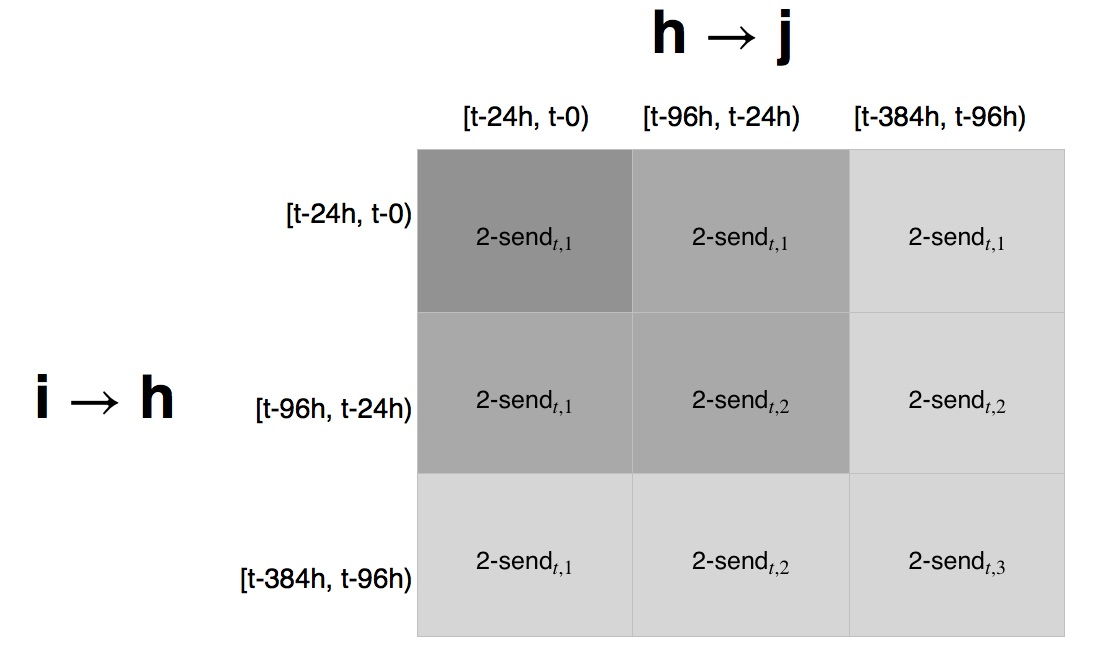
\includegraphics[width=0.6\textwidth]{triadtable.jpg} 
 	\label{fig:sim1diag}
 	\caption{Example of 2-send statistic defined for each interval $l=1,...,3$. Cells with same shades sum up to one statistic, based on when the triads are ``closed".}
 \end{figure}
In this setting, $\boldsymbol{x}^{(c)}_{t}(i, j)$ consists of:
\begin{verbatim}
"intercept"    
"outdegree1"   "outdegree2"   "outdegree3"   "indegree1"    "indegree2"    "indegree3"   
"send1"        "send2"        "send3"        "receive1"     "receive2"     "receive3"     
"2-send1"      "2-send2"      "2-send3"      "2-receive1"   "2-receive2"   "2-receive3"  
"sibling1"     "sibling2"     "sibling3"     "cosibling1"   "cosibling2"   "cosibling3"   
\end{verbatim}
and the corresponding dimension of  $\boldsymbol{b}^{(c)}$ becomes $P =  1 + 8 \times 3= 25$ for each interaction pattern $c=1,...,C$.
\subsection{Joint Generative Process of Document} \label{subsec: Joint Generative Process of Document}
 Below are the joint generative process for each document in a corpus $D$, integrating \ref{subsec: Content Generating Process}, \ref{subsec: Stochastic Intensity}, \ref{subsec: Tie Generating Process}, and \ref{subsec: Dynamic covariates2}.  Figure 1 is the corresponding plate notation of IPTM.
\begin{algorithm}[H]
	\SetAlgoLined
	\caption{Topic Word Distributions}
	\For{k=1 to K}{
		draw $\boldsymbol{\phi}^{(k)}$ $\sim$ Dir($\beta, \bf u$)
	}
\end{algorithm}
\begin{algorithm}[H]
	\SetAlgoLined
	\caption{Interaction Pattern Parameters}
	\For{c=1 to C}{
		draw $\boldsymbol{b}^{(c)}\sim \mbox{Normal}(\textbf{0}, \sigma^2I_P)$
	}
\end{algorithm}
\begin{algorithm}[H]
	\SetAlgoLined
	\caption{Topic Interaction Pattern Assginments}
	\For{k=1 to K}{
		draw $C_k$ $\sim$ Unif(1, C)
	}
\end{algorithm}
	\begin{algorithm}[H]
		\SetAlgoLined
		\caption{Document Generating Process}
		\For{d=1 to D}{
			draw $N^{(d)}= \mbox{max}(1, \bar N^{(d)})$, where $\bar N^{(d)}\sim \mbox{Poisson}(\zeta) $\\
			draw $\boldsymbol{\theta}^{(d)}\sim \mbox{Dir}(\alpha, \boldsymbol{m})$\\
				\For{n=1 to ${N}^{(d)}$}{
					draw $z_n^{(d)} \sim \mbox{Multinom}(\boldsymbol{\theta}^{(d)})$\\
					\If {$\bar N^{(d)}>0$} {
							draw $w_n^{(d)} \sim\mbox{Multinom} (\boldsymbol{\phi}^{(z_n^{(d)})})$
				}
			}
                   \For{c=1 to $C$}{
                   set $p_c^{(d)} = \frac{\sum\limits_{k: c_k=c} N^{(k|d)}}{N^{(d)}}$
                   }

                    \For{i=1 to $A$}{
                    	\For{j=1 to $A$}{
                    		\If {j $\neq$ i} {
                    			  calculate $\boldsymbol{x}_{t_+^{(d-1)}}^{(c)}(i, j)$, the network statisitcs evaluated at time $t_+^{(d-1)}$  \\
                    			  set $\lambda^{(d)}_{ij}=\sum\limits_{c=1}^{C} p^{(d)}_c\cdot\mbox{exp}\Big\{\boldsymbol{b}^{(c)T}\boldsymbol{x}^{(c)}_{t^{(d-1)}_+}(i, j)\Big\}\cdot 1\{j \in \mathcal{A}_{\backslash i}\}$\\
                        draw I($i \rightarrow j$) $\sim \mbox{Ber}(\frac{\delta\lambda^{(d)}_{ij}}{\delta\lambda^{(d)}_{ij}+1})$}  }
					draw $\Delta T_{iJ_i} \sim \mbox{Exp}(\lambda_{iJ_i}^{(d)})$
                    }
                    set $t^{(d)} = t^{(d-1)}+\mbox{min}(\Delta T_{i{J_i}})$, $i^{(d)} = i_{\mbox{min}(\Delta T_{i{J_i}})}$, and $J^{(d)} = J_{i^{(d)}}$
	}
	\end{algorithm}
	\subsection{Joint Generative Process of Document} \label{subsec: Joint Generative Process of Document}
	Below are the joint generative process for each document in a corpus $D$, integrating \ref{subsec: Content Generating Process}, \ref{subsec: Stochastic Intensity}, \ref{subsec: Tie Generating Process}, and \ref{subsec: Dynamic covariates2}.  Figure 1 is the corresponding plate notation of IPTM.
	\begin{algorithm}[H]
		\SetAlgoLined
		\caption{Topic Word Distributions}
		\For{k=1 to K}{
			draw $\boldsymbol{\phi}^{(k)}$ $\sim$ Dir($\beta, \bf u$)
		}
	\end{algorithm}
	\begin{algorithm}[H]
		\SetAlgoLined
		\caption{Interaction Pattern Parameters}
		\For{c=1 to C}{
			draw $\boldsymbol{b}^{(c)}\sim \mbox{Normal}(\textbf{0}, \sigma^2I_P)$
		}
	\end{algorithm}
	\begin{algorithm}[H]
		\SetAlgoLined
		\caption{Topic Interaction Pattern Assginments}
		\For{k=1 to K}{
			draw $C_k$ $\sim$ Unif(1, C)
		}
	\end{algorithm}
	\begin{algorithm}[H]
		\SetAlgoLined
		\caption{Document Generating Process}
		\For{d=1 to D}{
			draw $N^{(d)}= \mbox{max}(1, \bar N^{(d)})$, where $\bar N^{(d)}\sim \mbox{Poisson}(\zeta) $\\
			draw $\boldsymbol{\theta}^{(d)}\sim \mbox{Dir}(\alpha, \boldsymbol{m})$\\
			\For{n=1 to ${N}^{(d)}$}{
				draw $z_n^{(d)} \sim \mbox{Multinom}(\boldsymbol{\theta}^{(d)})$\\
				\If {$\bar N^{(d)}>0$} {
					draw $w_n^{(d)} \sim\mbox{Multinom} (\boldsymbol{\phi}^{(z_n^{(d)})})$
				}
			}
			\For{c=1 to $C$}{
				set $p_c^{(d)} = \frac{\sum\limits_{k: c_k=c} N^{(k|d)}}{N^{(d)}}$
			}
			
			\For{i=1 to $A$}{
				\For{j=1 to $A$}{
					\If {j $\neq$ i} {
						calculate $\boldsymbol{x}_{t_+^{(d-1)}}^{(c)}(i, j)$, the network statisitcs evaluated at time $t_+^{(d-1)}$  \\
						set $\lambda^{(d)}_{ij}=\sum\limits_{c=1}^{C} p^{(d)}_c\cdot\mbox{exp}\Big\{\boldsymbol{b}^{(c)T}\boldsymbol{x}^{(c)}_{t^{(d-1)}_+}(i, j)\Big\}\cdot 1\{j \in \mathcal{A}_{\backslash i}\}$\\
						draw I($i \rightarrow j$) $\sim \mbox{Ber}(\frac{\delta\lambda^{(d)}_{ij}}{\delta\lambda^{(d)}_{ij}+1})$}  }
				draw $\Delta T_{iJ_i} \sim \mbox{Exp}(\lambda_{iJ_i}^{(d)})$
			}
			set $t^{(d)} = t^{(d-1)}+\mbox{min}(\Delta T_{i{J_i}})$, $i^{(d)} = i_{\mbox{min}(\Delta T_{i{J_i}})}$, and $J^{(d)} = J_{i^{(d)}}$
		}
	\end{algorithm}
	\iffalse
	  \begin{figure}[ht]
	  	\centering
	  	\scalebox{0.6}{  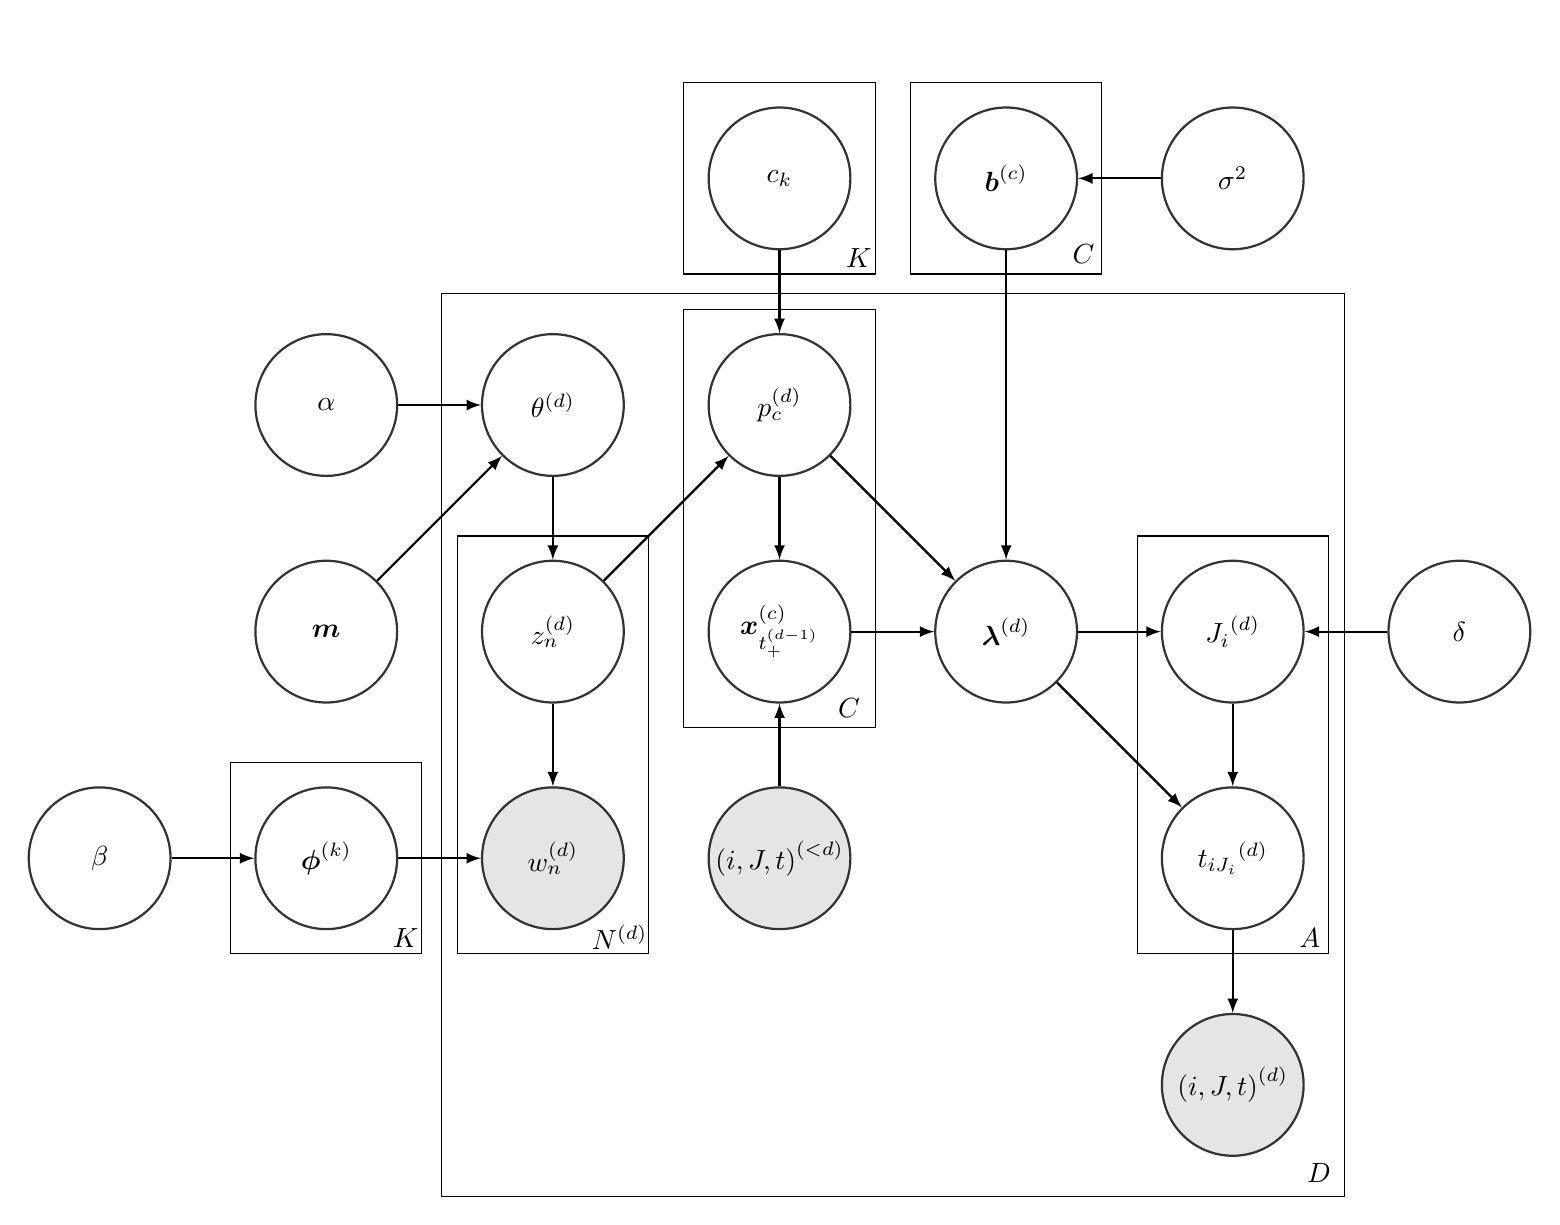
\begin{tikzpicture}
	  		\tikzstyle{main}=[circle, minimum size = 18mm, thick, draw =black!80, node distance = 10.5mm]
	  		\tikzstyle{connect}=[-latex, thick]
	  		\tikzstyle{box}=[rectangle, draw=black!100]
	  		\node[main] (theta) [label=center:${\theta}^{(d)}$] { };
	  		\node[main] (alpha) [left=of theta,label=center:${\alpha}$] { };
	  		\node[main] (z) [below=of theta,label=center:$z_n^{(d)}$] {};
	  		\node[main, fill = black!10] (w) [below=of z,label=center:$w_n^{(d)}$] { };
	  		\node[main] (phi) [left=of w,label=center:$\boldsymbol{\phi}^{(k)}$] { };
	  		\node[main] (beta) [left=of phi, label=center:$\beta$] { };
	  		\node[main] (m) [below=of alpha,label=center:$\boldsymbol{m}$] { };
	  		\node[main] (p) [right=of theta,label=center:$p_c^{(d)}$] { };
	  		\node[main] (x) [below=of p,label=center:$\boldsymbol{x}^{(c)}_{t_+^{(d-1)}}$] { };
	  		\node[main] (lambda) [right=of x,label=center:$\boldsymbol{\lambda}^{(d)}$] { };
	  		\node[main] (c) [above=of p,label=center:$c_k$] { };
	  		\node[main] (e) [right=of lambda,label=center:${J_i}^{(d)}$] { };
	  		\node[main] (delta) [right=of e,label=center:$\delta$] { };
	  		\node[main] (b) [right=of c,label=center:$\boldsymbol{b}^{(c)}$] { };
	  		\node[main] (t) [below=of e,label=center:${t_{iJ_i}}^{(d)}$] { };
	  		\node[main] (sigma) [right=of b,label=center:$\sigma^2$] { };
	  		\node[main, fill = black!10] (N) [below=of t,label=center:${(i, J, t)}^{(d)}$] { };
	  			\node[main, fill = black!10] (H) [below=of x,label=center:${(i, J, t)}^{(<d)}$] { };
	  		\path 
	  		(theta) edge [connect] (z)
	  		(z) edge [connect] (w)
	  		(alpha) edge [connect] (theta)
	  		(phi) edge [connect] (w)
	  		(beta) edge [connect] (phi)
	  		(z) edge [connect] (p)
	  		(x) edge [connect] (lambda)
	  		(c) edge [connect] (p)
	  		(p) edge [connect] (x)
	  		(p) edge [connect] (lambda)
	  		(b) edge [connect] (lambda)
	  		(lambda) edge [connect] (e)
	  		(lambda) edge [connect] (t)
	  		(sigma) edge [connect] (b)
	  		(e) edge [connect] (t)
	  		(delta) edge [connect] (e)
	  		(t) edge [connect] (N)
	  		(m) edge [connect] (theta)
	  		(H) edge [connect] (x);
	  		\node[rectangle, inner sep=5mm, draw=black!100, fit =(z) (w) (x) (theta) (N) (e)(lambda) ] {};
	  		\node[rectangle, inner sep=2mm, fit=(N),label=below right:$D$, xshift=-3mm, yshift=2.5mm] {};
	  		\node[rectangle, inner sep=3mm, draw=black!100, fit= (phi)] {};
	  		\node[rectangle, inner sep=3mm, draw=black!100, fit= (c)] {};
	  		\node[rectangle, inner sep=3mm,draw=black!100, fit= (b)] {};
	  		\node[rectangle, inner sep=4mm, fit= (b),label= below right:$C$, xshift=-6mm, yshift=6mm] {};
	  		\node[rectangle, inner sep=3mm,draw=black!100, fit= (x)(p)] {};
	  		\node[rectangle, inner sep=3mm, fit= (x),label= below right:$C$, xshift=-6mm, yshift=5mm] {};
	  		\node[rectangle, inner sep=0mm, fit= (phi),label=below right:$K$, xshift=-2mm, yshift=1.5mm] {};
	  		\node[rectangle, inner sep=0mm, fit= (c),label=below right:$K$, xshift=-2mm, yshift=1.5mm] {};
	  		\node[rectangle, inner sep=3mm,draw=black!100, fit= (w)(z)] {};
	  		\node[rectangle, inner sep=0mm, fit= (w),label=below right:$N^{(d)}$, xshift=-5.5mm, yshift=2mm] {};
	  		\node[rectangle, inner sep=3mm,draw=black!100, fit= (e)(t)] {};
	  		\node[rectangle, inner sep=0mm, fit=(t),label=below right:$A$, xshift=-2mm, yshift=1.5mm] {};
	  		\end{tikzpicture}}
	  	\caption{Plate notation of IPTM}
	  	\label{fig:plate}
	  \end{figure}
	  \fi
	\section{Inference} \label{sec: Inference}
	  The joint generative process implies a particular factorization of the joint distribution over the variables $\Phi=\{\boldsymbol{\phi}^{(k)}\}_{k=1}^{K}, \Theta=\{\boldsymbol{\theta}^{(d)} \}_{d=1}^{D},\mathcal{Z}=\{\boldsymbol{z}^{(d)} \}_{d=1}^{D},  \mathcal{W}=\{\boldsymbol{w}^{(d)} \}_{d=1}^{D}, \mathcal{C}=\{{c}_k \}_{k=1}^{K}, \mathcal{B}=\{\boldsymbol{b}^{(c)} \}_{c=1}^{C}, \mathcal{J}=\{\{J^{(d)}_i\}_{i=1}^{A}\}_{d=1}^D,\mathcal{T}=\{  \{t_{iJ_i}^{(d)}\}_{i=1}^{A}\}_{d=1}^D$, and $\mathcal{P}=\{(i, J, t)^{(d)}\}_{d=1}^D$ given the observed $\mathcal{P}^{\prime}=\{\{(i, J, t)^{(d^\prime)}\}_{d^\prime=1}^d\}_{d=1}^D$ and the hyperparameters $(\beta, \boldsymbol{u}, \alpha, \boldsymbol{m}, \sigma^2,  \delta)$:
	  \begin{equation}
	  \begin{aligned}
	  &P(\Phi, \Theta, \mathcal{Z}, \mathcal{W}, \mathcal{C}, \mathcal{B},\mathcal{J}, \mathcal{T}, \mathcal{P}|\mathcal{P}^{\prime}, \beta, \boldsymbol{u}, \alpha, \boldsymbol{m}, \sigma^2, \delta) \\& 
	  = P(\Phi|\beta, \boldsymbol{u})P(\Theta|\alpha, \boldsymbol{m})P(\mathcal{Z}|\Theta)P(\mathcal{W}|\mathcal{Z}, \Phi) P(\mathcal{C})P(\mathcal{B}|\mathcal{C}, \sigma^2)\\&\quad \quad \times
	  P(\mathcal{J}| \mathcal{Z}, \mathcal{C}, \mathcal{B}, \mathcal{P}^{\prime}, \delta)P(\mathcal{T}|\mathcal{Z}, \mathcal{C}, \mathcal{B}, \mathcal{J},  \mathcal{P}^{\prime})P(\mathcal{P}|\mathcal{J},\mathcal{T}, \mathcal{P}^{\prime}).
	  \end{aligned}
	  \end{equation}
	  We can simplify this further by integreting out $\Phi$ and $\Theta$ using Dirichlet-multinomial conjugacy:
	  \begin{equation}
	  \begin{aligned}
	  &P(\mathcal{Z}, \mathcal{W}, \mathcal{C}, \mathcal{B},\mathcal{J}, \mathcal{T}, \mathcal{P}|\mathcal{P}^{\prime}, \beta, \boldsymbol{u}, \alpha, \boldsymbol{m}, \sigma^2, \delta) \\& 
	  = P(\mathcal{Z}|\alpha, \boldsymbol{m})P(\mathcal{W}|\mathcal{Z}, \beta, \boldsymbol{u} ) P(\mathcal{C})P(\mathcal{B}|\mathcal{C}, \sigma^2)  P(\mathcal{J}| \mathcal{Z}, \mathcal{C}, \mathcal{B}, \mathcal{P}^{\prime}, \delta)P(\mathcal{T}|\mathcal{Z}, \mathcal{C}, \mathcal{B}, \mathcal{J},\mathcal{P}^{\prime})P(\mathcal{P}|\mathcal{J}, \mathcal{T}, \mathcal{P}^{\prime}).
	  \end{aligned}
	  \end{equation}
	  Note that since $p_c^{(d)}$ is a deterministic function of $(\mathcal{Z}, \mathcal{C})$, $\boldsymbol{x}_{t_+^{(d-1)}}^{(c)}$ is a deterministic function of $(p_c^{(d)}, \mathcal{P}^{\prime})$  and $\boldsymbol{\lambda}^{(d)}$ is a deterministic function of $(p_c^{(d)}, \boldsymbol{x}_{t_+^{(d-1)}}^{(c)}, \mathcal{B})$, we do not include them as variables in the joint distribution. \\ \newline
	 What we observe in the data is $\mathcal{W}$ and $\mathcal{P}$. We want to infer the values of all the latent variables ($\mathcal{Z}, \mathcal{C}, \mathcal{B}$) that most likely would have generated the data we observe, if we believe the generative process. Currently the variables ($\mathcal{J}, \mathcal{T}, \mathcal{P}, \mathcal{P^\prime}$) are redundant, thus we re-define the variables considering the data augmentation:  \iffalse  $\mathcal{I}_{\mbox{a}}=\{\{i^{(d)}\}_{i\neq i_o^{(d)}}\}_{d=1}^D,$  \fi $\mathcal{J}_{\mbox{a}}=\{\{J_i^{(d)}\}_{i\neq i_o^{(d)}}\}_{d=1}^D$, and $\mathcal{T}_{\mbox{a}}=\{\{t_{iJ_i}^{(d)}\}_{i\neq i_o^{(d)}}\}_{d=1}^D$ of the augmented data and $\mathcal{I}_{\mbox{o}}=\{i_o^{(d)}\}_{d=1}^D$,  $\mathcal{J}_{\mbox{o}}=\{J_o^{(d)}\}_{d=1}^D$, and $\mathcal{T}_{\mbox{o}}= \{t^{(d)}\}_{d=1}^D$ from the observed data.\\ \newline
	  Now, our inference goal is to draw samples from the posterior distribution
	  \begin{equation}
	  \begin{aligned}
	  &P(\mathcal{Z}, \mathcal{C}, \mathcal{B}, \mathcal{J}_{\mbox{a}}, \mathcal{T}_{\mbox{a}}|\mathcal{W}, \mathcal{I}_{\mbox{o}}, \mathcal{J}_{\mbox{o}}, \mathcal{T}_{\mbox{o}}, \beta, \boldsymbol{u}, \alpha, \boldsymbol{m}, \sigma^2,  \delta) \\
	  &\propto 	P(\mathcal{Z}, \mathcal{C}, \mathcal{B}, \mathcal{W}, \mathcal{J}_{\mbox{a}}, \mathcal{T}_{\mbox{a}},\mathcal{I}_{\mbox{o}}, \mathcal{J}_{\mbox{o}}, \mathcal{T}_{\mbox{o}} |\beta, \boldsymbol{u}, \alpha, \boldsymbol{m}, \sigma^2, \delta)\\&  = P(\mathcal{Z}|\alpha, \boldsymbol{m})P(\mathcal{C})P(\mathcal{B}|\mathcal{C}, \sigma^2)P(\mathcal{W}|\mathcal{Z}, \beta, \boldsymbol{u})P(\mathcal{J}_{\mbox{a}}, \mathcal{T}_{\mbox{a}},\mathcal{I}_{\mbox{o}}, \mathcal{J}_{\mbox{o}}, \mathcal{T}_{\mbox{o}} |\mathcal{Z}, \mathcal{C}, \mathcal{B}, \delta)
	  \end{aligned}
	  \end{equation}
  As mentioned earlier in Section \ref{subsec: Tie Generating Process}, we use data augmentation in the tie generating process. Since we should include both the observed and augmented data to make inferences on the related latent variables, the derivation steps for the contribution of tie is not as smiple as other variables. Therefore, here we provide the detailed derivation steps for the last term of conditional probability: 
 \begin{equation}
\begin{aligned}
&P(\mathcal{J}_{\mbox{a}}, \mathcal{T}_{\mbox{a}},\mathcal{I}_{\mbox{o}}, \mathcal{J}_{\mbox{o}}, \mathcal{T}_{\mbox{o}} |\mathcal{Z}, \mathcal{C}, \mathcal{B}, \delta)\\& = \prod_{d=1}^D P(\mathcal{J}^{(d)}_{\mbox{a}}, \mathcal{T}^{(d)}_{\mbox{a}}, i^{(d)}_{\mbox{o}}, J^{(d)}_{\mbox{o}}, t^{(d)}_{\mbox{o}} |\mathcal{I}^{(<d)}_{\mbox{o}}, \mathcal{J}^{(<d)}_{\mbox{o}}, \mathcal{T}^{(<d)}_{\mbox{o}},\mathcal{Z}, \mathcal{C}, \mathcal{B}, \delta).
\end{aligned}
 \end{equation}
Now we tackle the problem by deriving $P(\mathcal{J}^{(d)}_{\mbox{a}}, \mathcal{T}^{(d)}_{\mbox{a}}, i^{(d)}_{\mbox{o}}, J^{(d)}_{\mbox{o}}, t^{(d)}_{\mbox{o}} |\mathcal{I}^{(<d)}_{\mbox{o}}, \mathcal{J}^{(<d)}_{\mbox{o}}, \mathcal{T}^{(<d)}_{\mbox{o}}, \mathcal{Z}, \mathcal{C}, \mathcal{B}, \delta)$ for $d^{th}$ document. There are three steps involved. First is the generation of the latent receivers $J_i$ for each $i$, which corresponds to the Bernoulli part of tie generation, Equation (5); second is the generation of the observed time increment $\Delta T^{(d)} = t^{(d)} - t^{(d-1)}$ from the observed sender-receiver pairs ($i^{(d)}_{\mbox{o}}, J^{(d)}_{\mbox{o}}$), which corresponds to the Exponential part of tie generation in Equation (6); and the last part is the simultaneous selection process of the observed sender, receivers, and timestamp in Equation (7), implying that the latent time increments generated from the latent sender-receiver pairs were greater than the observed time increment $t^{(d)} - t^{(d-1)}$. Reflecting the three steps, the joint distribution is:\\
  \begin{equation},
  \begin{aligned}
&P(\mathcal{J}^{(d)}_{\mbox{a}}, \mathcal{T}^{(d)}_{\mbox{a}}, i^{(d)}_{\mbox{o}}, J^{(d)}_{\mbox{o}}, t^{(d)}_{\mbox{o}} |\mathcal{I}^{(<d)}_{\mbox{o}}, \mathcal{J}^{(<d)}_{\mbox{o}}, \mathcal{T}^{(<d)}_{\mbox{o}}, \mathcal{Z}, \mathcal{C}, \mathcal{B}, \delta)\\&= P\Big(\mathcal{J}^{(d)}_{\mbox{a}}, J^{(d)}_{\mbox{o}}| i^{(d)}_{\mbox{o}}, \mathcal{I}^{(<d)}_{\mbox{o}}, \mathcal{J}^{(<d)}_{\mbox{o}}, \mathcal{T}^{(<d)}_{\mbox{o}}, \mathcal{Z}, \mathcal{C}, \mathcal{B}, \delta\Big) \times P\Big(t^{(d)}_{\mbox{o}} |i^{(d)}_{\mbox{o}}, J^{(d)}_{\mbox{o}}, \mathcal{I}^{(<d)}_{\mbox{o}}, \mathcal{J}^{(<d)}_{\mbox{o}}, \mathcal{T}^{(<d)}_{\mbox{o}}, \mathcal{Z}, \mathcal{C}, \mathcal{B}\Big)\\& \times P\Big( \mathcal{T}^{(d)}_{\mbox{a}} >t^{(d)}_{\mbox{o}} |\mathcal{J}^{(d)}_{\mbox{a}}, i^{(d)}_{\mbox{o}}, t^{(d)}_{\mbox{o}}, \mathcal{I}^{(<d)}_{\mbox{o}}, \mathcal{J}^{(<d)}_{\mbox{o}}, \mathcal{T}^{(<d)}_{\mbox{o}}, \mathcal{Z}, \mathcal{C}, \mathcal{B}\Big) \\&
=\prod_{i\in \mathcal{A}}\prod_{j\in \mathcal{A}_{\backslash i}}\Big(I(i \rightarrow j)\sim \mbox{Ber}(\frac{\delta\lambda^{(d)}_{ij}}{\delta\lambda^{(d)}_{ij}+1})\Big) \times \Big(\Delta T^{(d)}\sim\mbox{Exp}(\lambda^{(d)}_{i_o^{(d)}J_{o}^{(d)}})\Big) \times \prod_{i\in \mathcal{A}_{\backslash i_o^{(d)}}}P\Big(\Delta T^{(d)}_{i{J^{(d)}_i}} > \Delta T^{(d)}\Big)\\&
=\Big(\prod_{i\in \mathcal{A}}\prod_{j \in \mathcal{A}_{\backslash i }} \big(\frac{\delta\lambda^{(d)}_{ij}}{\delta\lambda^{(d)}_{ij}+1}\big)^{I(j \in J^{(d)}_i)}\big(\frac{1}{\delta\lambda^{(d)}_{ij}+1}\big)^{1-I(j \in J^{(d)}_i)}\Big)\times \Big(\lambda^{(d)}_{i_o^{(d)}J_{o}^{(d)}}e^{-(t^{(d)}-t^{(d-1)})\lambda^{(d)}_{i_o^{(d)}J_{o}^{(d)}}}\Big)\\ &\times  \prod_{i\in \mathcal{A}_{\backslash i_o^{(d)}}}\Big(e^{-(t^{(d)}-t^{(d-1)})\lambda^{(d)}_{iJ^{(d)}_{i}}}\Big),
  \end{aligned}
  \end{equation}
  where the last term is given by the cumulative exponential distributions associated with the respective $\lambda^{(d)}_{iJ_i}$. Therefore, we can simplify the above equation as below:
  \begin{equation}
  \begin{aligned}
  &P(\mathcal{J}^{(d)}_{\mbox{a}}, \mathcal{T}^{(d)}_{\mbox{a}}, i^{(d)}_{\mbox{o}}, J^{(d)}_{\mbox{o}}, t^{(d)}_{\mbox{o}} |\mathcal{I}^{(<d)}_{\mbox{o}}, \mathcal{J}^{(<d)}_{\mbox{o}}, \mathcal{T}^{(<d)}_{\mbox{o}}, \mathcal{Z}, \mathcal{C}, \mathcal{B}, \delta)\\&=\Big(\prod_{i\in \mathcal{A}}\prod_{j \in \mathcal{A}_{\backslash i }} \frac{(\delta\lambda^{(d)}_{ij})^{I(j \in J_i)}}{\delta\lambda^{(d)}_{ij}+1}\Big)\times \Big(\lambda^{(d)}_{i_o^{(d)}J_{o}^{(d)}}\Big)\times  \Big(e^{-(t^{(d)}-t^{(d-1)})\sum\limits_{i\in \mathcal{A}_{\backslash J^{(d)}_i = \emptyset}}\lambda^{(d)}_{iJ^{(d)}_{i}}}\Big).
  \end{aligned}
  \end{equation}
For implementation, we need to compute these equations in log space to prevent underflow:
 \begin{equation}
 \begin{aligned}
 &\mbox{log}\Big(P(\mathcal{J}^{(d)}_{\mbox{a}}, \mathcal{T}^{(d)}_{\mbox{a}}, i^{(d)}_{\mbox{o}}, J^{(d)}_{\mbox{o}}, t^{(d)}_{\mbox{o}} |\mathcal{I}^{(<d)}_{\mbox{o}}, \mathcal{J}^{(<d)}_{\mbox{o}}, \mathcal{T}^{(<d)}_{\mbox{o}}, \mathcal{Z}, \mathcal{C}, \mathcal{B},  \delta)\Big)\\&=\Big(\sum_{i\in \mathcal{A}}\sum_{j \in \mathcal{A}_{\backslash i }} {I(j \in J_i)}\cdot\mbox{log}(\delta\lambda^{(d)}_{iJ_i}) {-\mbox{log}(\delta\lambda^{(d)}_{ij}}+1)\Big)+ \Big(\mbox{log}(\lambda^{(d)}_{i_o^{(d)}J_o^{(d)}})\Big) {-\Big((t^{(d)}-t^{(d-1)})\sum\limits_{i \in \mathcal{A}_{\backslash J_i^{(d)}=\emptyset}}\lambda^{(d)}_{i{J_i^{(d)}}}\Big)}.
 \end{aligned}
 \end{equation}
 To actually perform inference, we therefore want to use Gibbs sampling, where we will sequentially resample the values of each of our latent variables from their posterior distribution, conditional on all of our other variables.
    \subsection{Resampling the augmented data $\mathcal{J}_a$} \label{subsec: Data augmentation}
      First of all, for each document $d$, we update the latent sender-receiver(s) pairs. That is, given the observed sender of the document $i_o^{(d)}$, we sample the latent receivers for each sender except the observed. Here we illustrate how each sender-receiver pair in the document $d$ is updated.\\\newline
      Define $\boldsymbol{r}^{(d)}_i = (r_{i1},..., r_{iA})^{(d)}$ be the $(A-1)$ length vector of indicators (0/1) representing the latent receivers corresponding to the sender $i$ in the docuemnt $d$. Here, for each sender $i$ and receiver  $j \in \mathcal{A}_{\backslash i}$, we are going to resample each $r_{ij}$, one at a time.\\
      \begin{equation}
      \begin{aligned}
      &P(\mathcal{J}^{(d)}_{\mbox{a}}=\{\boldsymbol{r}^{(d)}_i\}_{i\in \mathcal{A}_{\backslash i_o^{(d)}}}| i^{(d)}_{\mbox{o}}, J^{(d)}_{\mbox{o}}, t^{(d)}_{\mbox{o}}, \mathcal{T}^{(d)}_{\mbox{a}}, \mathcal{I}^{(<d)}_{\mbox{o}}, \mathcal{J}^{(<d)}_{\mbox{o}}, \mathcal{T}^{(<d)}_{\mbox{o}}, \mathcal{Z}, \mathcal{C}, \mathcal{B}, \delta)\\&\propto P(\mathcal{J}^{(d)}_{\mbox{a}}=\{\boldsymbol{r}^{(d)}_i\}_{i\in \mathcal{A}_{\backslash i_o^{(d)}}}, \mathcal{T}^{(d)}_{\mbox{a}}| i^{(d)}_{\mbox{o}}, J^{(d)}_{\mbox{o}}, t^{(d)}_{\mbox{o}},  \mathcal{I}^{(<d)}_{\mbox{o}}, \mathcal{J}^{(<d)}_{\mbox{o}}, \mathcal{T}^{(<d)}_{\mbox{o}}, \mathcal{Z}, \mathcal{C}, \mathcal{B}, \delta)\\&=\prod\limits_{i \in \mathcal{A}_{\backslash i_o^{(d)}}}\Big(P(J_i^{(d)}=\boldsymbol{r}_i^{(d)}|i^{(d)}_{\mbox{o}}, \mathcal{I}^{(<d)}_{\mbox{o}}, \mathcal{J}^{(<d)}_{\mbox{o}}, \mathcal{T}^{(<d)}_{\mbox{o}}, \mathcal{Z}, \mathcal{C}, \mathcal{B}, \delta)\\&\quad\quad\quad\quad\quad\times P(\Delta T^{(d)}_{iJ_i^{(d)}} >\Delta T^{(d)}| J_i^{(d)} =\boldsymbol{r}^{(d)}_i , t^{(d)}_{\mbox{o}}, \mathcal{I}^{(<d)}_{\mbox{o}}, \mathcal{J}^{(<d)}_{\mbox{o}}, \mathcal{T}^{(<d)}_{\mbox{o}}, \mathcal{Z}, \mathcal{C}, \mathcal{B})\Big)\\&
      =\prod\limits_{i \in \mathcal{A}_{\backslash i_o^{(d)}}}\Big(\prod\limits_{j \in \mathcal{A}_{\backslash i}}P(J_{ij}^{(d)}={r}_{ij}^{(d)}| J_{i_{\backslash j}}^{(d)}=\boldsymbol{r}^{(d)}_{i_{\backslash j}} , i^{(d)}_{\mbox{o}}, \mathcal{I}^{(<d)}_{\mbox{o}}, \mathcal{J}^{(<d)}_{\mbox{o}}, \mathcal{T}^{(<d)}_{\mbox{o}}, \mathcal{Z}, \mathcal{C}, \mathcal{B}, \delta)\Big)\\&\quad\quad\quad\quad\quad\times P(\Delta T^{(d)}_{iJ_i^{(d)}} >\Delta T^{(d)}|J_{i}^{(d)} =\boldsymbol{r}^{(d)}_{i}  , t^{(d)}_{\mbox{o}}, \mathcal{I}^{(<d)}_{\mbox{o}}, \mathcal{J}^{(<d)}_{\mbox{o}}, \mathcal{T}^{(<d)}_{\mbox{o}}, \mathcal{Z}, \mathcal{C}, \mathcal{B}).
      \end{aligned}
      \end{equation}
      Then, since $r_{ij}^{(d)}$ could be either 1 or 0, we divide into two cases for the sampling of $j^{th}$ element of $J_i^{(d)}$, as below:
      \begin{equation}
      \begin{aligned}
      &P(J_{ij}^{(d)}=1|  J_{i_{\backslash j}}^{(d)}=\boldsymbol{r}^{(d)}_{i_{\backslash j}}, i^{(d)}_{\mbox{o}}, J^{(d)}_{\mbox{o}}, t^{(d)}_{\mbox{o}}, \mathcal{T}^{(d)}_{\mbox{a}},  \mathcal{I}^{(<d)}_{\mbox{o}}, \mathcal{J}^{(<d)}_{\mbox{o}}, \mathcal{T}^{(<d)}_{\mbox{o}}, \mathcal{Z}, \mathcal{C}, \mathcal{B}, \delta)\\&
      \propto P(J_{ij}^{(d)}=1|i^{(d)}_{\mbox{o}},\mathcal{I}^{(<d)}_{\mbox{o}}, \mathcal{J}^{(<d)}_{\mbox{o}}, \mathcal{T}^{(<d)}_{\mbox{o}}, \mathcal{Z}, \mathcal{C}, \mathcal{B}, \delta)\\&\times P(\Delta T^{(d)}_{iJ_i^{(d)}} >\Delta T^{(d)}|J_{ij}^{(d)} =1,  J_{i_{\backslash j}}^{(d)}=\boldsymbol{r}^{(d)}_{i_{\backslash j}}, t^{(d)}_{\mbox{o}}, \mathcal{I}^{(<d)}_{\mbox{o}}, \mathcal{J}^{(<d)}_{\mbox{o}}, \mathcal{T}^{(<d)}_{\mbox{o}}, \mathcal{Z}, \mathcal{C}, \mathcal{B})\\& =\frac{\delta\lambda^{(d)}_{ij}}{\delta\lambda^{(d)}_{ij}+1}\times e^{-(t^{(d)}-t^{(d-1)})\lambda^{(d)}_{iJ^{(d)}_{i[+j]}}},
      \end{aligned}
      \end{equation}
      where $\lambda^{(d)}_{iJ^{(d)}_{i[+j]}}$ meaning that preveiously defined $\lambda^{(d)}_{iJ^{(d)}_{i}}=\sum\limits_{c=1}^{C} p^{(d)}_c\cdot\mbox{exp}\Big\{\frac{1}{|J_i|}\sum\limits_{j \in{J_i}}\boldsymbol{b}^{(c)T}\boldsymbol{x}^{(c)}_{t^{(d-1)}_+}(i, j)\Big\}\cdot \prod\limits_{j \in J_i}1\{j \in \mathcal{A}_{\backslash i}\} $ is calculated with $j^{th}$ element of $J_i^{(d)}$ fixed as 1. On the other hand, 
       \begin{equation}
       \begin{aligned}
       &P(J_{ij}^{(d)}=0| J_{i_{\backslash j}}^{(d)}=\boldsymbol{r}^{(d)}_{i_{\backslash j}}, i^{(d)}_{\mbox{o}},J^{(d)}_{\mbox{o}}, t^{(d)}_{\mbox{o}}, \mathcal{T}^{(d)}_{\mbox{a}}, \mathcal{I}^{(<d)}_{\mbox{o}}, \mathcal{J}^{(<d)}_{\mbox{o}}, \mathcal{T}^{(<d)}_{\mbox{o}}, \mathcal{Z}, \mathcal{C}, \mathcal{B}, \delta)\\&
       \propto P(J_{ij}^{(d)}=0|i^{(d)}_{\mbox{o}},\mathcal{I}^{(<d)}_{\mbox{o}}, \mathcal{J}^{(<d)}_{\mbox{o}}, \mathcal{T}^{(<d)}_{\mbox{o}}, \mathcal{Z}, \mathcal{C}, \mathcal{B}, \delta)\\&\times P(\Delta T^{(d)}_{iJ_i^{(d)}} >\Delta T^{(d)}|J_{ij}^{(d)} =0,  J_{i_{\backslash j}}^{(d)}=\boldsymbol{r}^{(d)}_{i_{\backslash j}}, t^{(d)}_{\mbox{o}}, \mathcal{I}^{(<d)}_{\mbox{o}}, \mathcal{J}^{(<d)}_{\mbox{o}}, \mathcal{T}^{(<d)}_{\mbox{o}}, \mathcal{Z}, \mathcal{C}, \mathcal{B})\\& =\frac{1}{\delta\lambda^{(d)}_{ij}+1}\times e^{-(t^{(d)}-t^{(d-1)})\lambda^{(d)}_{iJ^{(d)}_{i[-j]}}},
       \end{aligned}
       \end{equation}
       where $\lambda^{(d)}_{iJ^{(d)}_{i[-j]}}$ meaning similarly as above that $\lambda^{(d)}_{iJ^{(d)}_{i}}=\sum\limits_{c=1}^{C} p^{(d)}_c\cdot\mbox{exp}\Big\{\frac{1}{|J_i|}\sum\limits_{j \in{J_i}}\boldsymbol{b}^{(c)T}\boldsymbol{x}^{(c)}_{t^{(d-1)}_+}(i, j)\Big\}\cdot \prod\limits_{j \in J_i}1\{j \in \mathcal{A}_{\backslash i}\} $ is calculated with $j^{th}$ element of $J_i^{(d)}$ fixed as 0. Now we can use Gibbs sampling using the two probabilities, Equation (16) and Equation (17). Note that we would calculate the equations in the log space to prevent from numerical underflow.
   \iffalse
   \subsection{Resampling the augmented data $\mathcal{J}_a$} \label{subsec: Data augmentation}
   First of all, for each document $d$, we update the latent sender and the corresponding receiver set,  $\mathcal{I}^{(d)}_{\mbox{a}}=\{i^{(d)}\}_{i\neq i^{(d)}}$ and  $\mathcal{J}^{(d)}_{\mbox{a}}=\{J_i^{(d)}\}_{i\neq i^{(d)}}$, by accounting for the conditional probability $P(\mbox{latent receivers}| \mbox{latent time} < \mbox{observed time})$. To derive this, let $\Delta T_{i_o^{(d)}{J_o^{(d)}}}$ be the observed time increment, and $\Delta T_{i_a{J_{i_a}}}$ be the latent time increment associated with the document sent by $i_a$. We also define $(i \rightarrow j)$ be an indicator of whether sender $i$ added $j$ to the latent receivers (i.e. $j \in J_i$), and $J_i^{(-j)}$ denote the vector of recipient indicators other than $j$. Then the conditional probability is:\\
   \begin{equation}
   	\begin{split}
   		&P\Big(i \to j|(\Delta T_{i{J_i}} > \Delta T_{i^{(d)}{J^{(d)}}})\cap( J_i^{(-j)})\Big)\\ &=\frac{P\Big((i \rightarrow j)\cap (\Delta T_{i{J_i}} > \Delta T_{i^{(d)}{J^{(d)}}})\cap (J_i^{(-j)})\Big)}{P\Big((\Delta T_{i{J_i}} > \Delta T_{i^{(d)}{J^{(d)}}})\cap (J_i^{(-j)})\Big)}\\
   		& = \frac{P\Big(\Delta T_{i{J_i}} > \Delta T_{i^{(d)}{J^{(d)}}} | (i \to j)\cap (J_i^{(-j)})\Big)P\Big((i \to j) \cap (J_i^{(-j)})\Big)}{P\Big((\Delta T_{i{J_i}} > \Delta T_{i^{(d)}{J^{(d)}}})\cap (J_i^{(-j)})|i \to j\Big)P\Big(i \to j\Big)+P\Big( (\Delta T_{i{J_i}} > \Delta T_{i^{(d)}{J^{(d)}}}) \cap (J_i^{(-j)})|i \not\to j\Big)P\Big(i \not\to j\Big)},
   	\end{split}
   \end{equation}
   where $P\Big(\Delta T_{i{J_i}} > \Delta T_{i^{(d)}{J^{(d)}}} | (i \rightarrow j)\cap (J_i^{(-j)})\Big)$, $P\Big((\Delta T_{i{J_i}}> \Delta T_{i^{(d)}{J^{(d)}}})\cap (J_i^{(-j)})|i \rightarrow j\Big)$, and $P\Big((\Delta T_{i{J_i}}> \Delta T_{i^{(d)}{J^{(d)}}})\cap (J_i^{(-j)})|i\not\to j\Big)$ are given by the cumulative exponential distributions associated with the respective $\lambda^{(d)}_{iJ_i}$ and $P\Big((i \rightarrow j) \cap (J_i^{(-j)})\Big)$,  $P\Big(i \rightarrow j\Big)$, and $P\Big(i\not\to j\Big)$ are given by the Bernoulli equation in Section \ref{subsec: Tie Generating Process}. We plug in the equations and update the latent ties $(i \rightarrow j)$ with the probability:
   \begin{equation}
   	\begin{split}
   		&P\Big(i \rightarrow j|(\Delta T_{i{J_i}} > \Delta T_{i^{(d)}{J^{(d)}}})\cap( J_i^{(-j)})\Big)
   		\\&=\frac{e^{-(t^{(d)}-t^{(d-1)})\frac{1}{|J_i^{(+j)}|}\sum\limits_{j \in J_i^{(+j)}}\lambda^{(d)}_{ij}}\times(\frac{\delta\lambda^{(d)}_{ij}}{\delta\lambda^{(d)}_{ij}+1})\times\Big(\prod_{a \in \mathcal{A}_{\backslash i, j}} {(\delta\lambda^{(d)}_{ij})}^{I(a \in J_i)} / (\delta\lambda^{(d)}_{ij}+1)\Big)}{e^{-(t^{(d)}-t^{(d-1)})\frac{1}{|J_i^{(+j)}|}\sum\limits_{j \in J_i^{(+j)}}\lambda^{(d)}_{ij}}\times(\frac{\delta\lambda^{(d)}_{ij}}{\delta\lambda^{(d)}_{ij}+1})+e^{-(t^{(d)}-t^{(d-1)})\frac{1}{|J_i^{(-j)}|}\sum\limits_{j \in J_i^{(-j)}}\delta\lambda^{(d)}_{ij}}\times(\frac{1}{\delta\lambda^{(d)}_{ij}+1})}
\\&=\frac{\Big(\prod_{a \in \mathcal{A}_{\backslash i, j}} {(\delta\lambda^{(d)}_{ij})}^{I(a \in J_i)} / (\delta\lambda^{(d)}_{ij}+1)\Big)}{1 + e^{(t^{(d)}-t^{(d-1)})\big(\frac{1}{|J_i^{(+j)}|}\sum\limits_{j \in J_i^{(+j)}}\lambda^{(d)}_{ij} -\frac{1}{|J_i^{(-j)}|}\sum\limits_{j \in J_i^{(-j)}}\lambda^{(d)}_{ij} \big)} / \delta\lambda^{(d)}_{ij}}.   	\end{split}
   \end{equation}
  This probability will be used when we update the augmented data in every outer iteration. For implementation, we need to compute these equations in log space:
  \begin{equation}
  \begin{aligned}
  &\mbox{log}\Big(P\Big(i\to j|(\Delta T_{i{J_i}} > \Delta T_{i^{(d)}{J^{(d)}}})\cap( J_i^{(-j)})\Big)\Big)\\&=\Big(\sum_{a \in \mathcal{A}_{\backslash i, j}} {{I(a \in J_i)}\cdot \mbox{log}(\delta\lambda^{(d)}_{ij})}- \mbox{log}(\delta\lambda^{(d)}_{ij}+1)\Big)\\&-\mbox{log}\Big(1 + e^{(t^{(d)}-t^{(d-1)})\big(\frac{1}{|J_i^{(+j)}|}\sum\limits_{j \in J_i^{(+j)}}\lambda^{(d)}_{ij} -\frac{1}{|J_i^{(-j)}|}\sum\limits_{j \in J_i^{(-j)}}\lambda^{(d)}_{ij} \big) - \mbox{log}(\delta\lambda^{(d)}_{ij})} \Big).   
  \end{aligned}
  \end{equation}
  Moreover, to further protect from numerical underflow and overflow, we use the numerical approximation of $f(y) = \mbox{log}(1+ e^y)$ as below: 
  \begin{equation*}
  f(y) = \begin{cases}
  y &y >35\\
  e^y & y<-10\\
  \mbox{log}(1+e^y) & \mbox{otherwise},
  \end{cases}
  \end{equation*}
  where $y = (t^{(d)}-t^{(d-1)})\big(\frac{1}{|J_i^{(+j)}|}\sum\limits_{j \in J_i^{(+j)}}\lambda^{(d)}_{ij} -\frac{1}{|J_i^{(-j)}|}\sum\limits_{j \in J_i^{(-j)}}\lambda^{(d)}_{ij} \big) - \mbox{log}(\delta\lambda^{(d)}_{ij})$ in this case.
  \fi
  \newpage
  \subsection{Resampling $\mathcal{Z}$}  \label{subsec: Resampling Z}
Second, we are going to resample the topic assignments, one words in a document at a time.  The new values of $z^{(d)}_n$ are sampled using the conditional posterior probability of being topic $k$ as we derived in APPENDIX C:
 \begin{equation}
 \begin{aligned} & 
 P(z^{(d)}_n=k|\mathcal{Z}_{\backslash d, n},   \mathcal{C},   \mathcal{B},\mathcal{W}, \mathcal{I}_{\mbox{a}}, \mathcal{J}_{\mbox{a}}, \mathcal{T}_{\mbox{a}}, \mathcal{I}_{\mbox{o}}, \mathcal{J}_{\mbox{o}}, \mathcal{T}_{\mbox{o}}, \beta, \boldsymbol{u}, \alpha, \boldsymbol{m}, \sigma^2, \delta)\\
 & \propto P(z^{(d)}_n=k, w^{(d)}_n, \mathcal{I}^{(d)}_{\mbox{a}}, \mathcal{J}^{(d)}_{\mbox{a}}, \mathcal{T}^{(d)}_{\mbox{a}}, \mathcal{I}^{(d)}_{\mbox{o}}, \mathcal{J}^{(d)}_{\mbox{o}}, \mathcal{T}^{(d)}_{\mbox{o}}|\mathcal{Z}_{\backslash d, n}, \mathcal{C},   \mathcal{B},\mathcal{W}_{\backslash d, n}, \mathcal{I}^{(-d)}_{\mbox{o}}, \mathcal{J}^{(-d)}_{\mbox{o}}, \mathcal{T}^{(-d)}_{\mbox{o}}, \beta, \boldsymbol{u}, \alpha, \boldsymbol{m}, \sigma^2, \delta)\\
 &=P(z^{(d)}_n=k|\mathcal{Z}_{\backslash d, n}, \alpha, \boldsymbol{m})P(w^{(d)}_n|z^{(d)}_n=k, \mathcal{W}_{\backslash d, n}, \mathcal{Z}_{\backslash d, n}, \beta, \boldsymbol{u} )\\&\quad\quad \times P(\mathcal{I}^{(d)}_{\mbox{a}}, \mathcal{J}^{(d)}_{\mbox{a}}, \mathcal{T}^{(d)}_{\mbox{a}}, \mathcal{I}^{(d)}_{\mbox{o}}, \mathcal{J}^{(d)}_{\mbox{o}}, \mathcal{T}^{(d)}_{\mbox{o}}| z^{(d)}_n=k, \mathcal{Z}_{\backslash d, n}, \mathcal{C}, \mathcal{B}, \sigma^2, \delta)
 \end{aligned}
 \end{equation}
 where the subscript $``{\backslash d, n}"$ denotes the exclsuion of position $n$ in $d^{th}$ document and the subscript $``{\backslash d}"$ and $``{(-d)}"$ denotes the exclsuion of $d^{th}$ document. We know that:
 \begin{equation}
 \begin{aligned} 
 P(z^{(d)}_n=k|\mathcal{Z}_{\backslash d, n}, \alpha, \boldsymbol{m})=\frac{N^{(k|d)}_{\backslash d, n}+\alpha \boldsymbol{m}_k}{N^{(d)}-1+\alpha}
 \end{aligned}
 \end{equation}
 which is the well-known form of collapsed Gibbs sampling equation for LDA. We also know that \begin{equation}
 \begin{aligned} 
 P(w^{(d)}_n|z^{(d)}_n=k, \mathcal{W}_{\backslash d, n}, \mathcal{Z}_{\backslash d, n}, \beta, \boldsymbol{u} )=\frac{N^{(w_n^{(d)}|k)}_{\backslash d, n}+\frac{\beta}{W} }{N^{(k)}_{\backslash d, n}+\beta},
 \end{aligned}
 \end{equation}
 where $N^{(w_n^{(d)}|k)}$ is the number of tokens assigned to topic $k$ whose type is the same as that of $w_n^{(d)}$, excluding $w_n^{(d)}$ itself, and $N^{(k)}_{\backslash d, n}=\sum_{w=1}^W N_{\backslash d, n}^{(w_n^{(d)}|k)}$. Finally, in \ref{subsec: Data augmentation}, we have shown that
 \begin{equation}
 \begin{aligned}
& P(\mathcal{I}^{(d)}_{\mbox{a}}, \mathcal{J}^{(d)}_{\mbox{a}}, \mathcal{T}^{(d)}_{\mbox{a}}, \mathcal{I}^{(d)}_{\mbox{o}}, \mathcal{J}^{(d)}_{\mbox{o}}, \mathcal{T}^{(d)}_{\mbox{o}}| z^{(d)}_n=k, \mathcal{Z}_{\backslash d, n}, \mathcal{C}, \mathcal{B}, \sigma^2, \delta)\\&=\Big(\prod_{i\in \mathcal{A}}\prod_{j \in \mathcal{A}_{\backslash i }} \frac{(\delta\lambda^{(d)}_{ij})^{I(j \in J_i)}}{\delta\lambda^{(d)}_{ij}+1}\Big)\times \Big(\lambda^{(d)}_{i_o^{(d)}J_{o}^{(d)}}\Big)\times  \Big(e^{-(t^{(d)}-t^{(d-1)})\sum\limits_{i\in \mathcal{A}_{\backslash J^{(d)}_i = \emptyset}}\lambda^{(d)}_{iJ^{(d)}_{i}}}\Big).
 \end{aligned}
 \end{equation}
 Therefore, if $\bar N^{(d)} > 0$, then
 \begin{equation}
 \begin{aligned}
  &P(z^{(d)}_n=k|\mathcal{Z}_{\backslash d, n},   \mathcal{C},   \mathcal{B},\mathcal{W}, \mathcal{I}_{\mbox{a}}, \mathcal{J}_{\mbox{a}}, \mathcal{T}_{\mbox{a}}, \mathcal{I}_{\mbox{o}}, \mathcal{J}_{\mbox{o}}, \mathcal{T}_{\mbox{o}}, \beta, \boldsymbol{u}, \alpha, \boldsymbol{m}, \sigma^2, \delta)\\&\propto (N^{(k|d)}_{\backslash d, n}+\alpha \boldsymbol{m}_k)\times \frac{N^{(w_n^{(d)}|k)}_{\backslash d, n}+\frac{\beta}{W} }{N^{(k)}_{\backslash d, n}+\beta}\times\Big(\prod_{i\in \mathcal{A}}\prod_{j \in \mathcal{A}_{\backslash i }} \frac{(\delta\lambda^{(d)}_{ij})^{I(j \in J_i)}}{\delta\lambda^{(d)}_{ij}+1}\Big)\times \Big(\lambda^{(d)}_{i_o^{(d)}J_{o}^{(d)}}\Big)\times  \Big(e^{-(t^{(d)}-t^{(d-1)})\sum\limits_{i\in \mathcal{A}_{\backslash J^{(d)}_i = \emptyset}}\lambda^{(d)}_{iJ^{(d)}_{i}}}\Big), 
 \end{aligned}
 \end{equation}
 and if $\bar N^{(d)} = 0$, then the first term becomes $\alpha\boldsymbol{m_k}$ and disappears because it is a constant. The second term disappears since there are no tokens, thus we just have the last three terms, $P(\mathcal{I}^{(d)}_{\mbox{a}}, \mathcal{J}^{(d)}_{\mbox{a}}, \mathcal{T}^{(d)}_{\mbox{a}}, \mathcal{I}^{(d)}_{\mbox{o}}, \mathcal{J}^{(d)}_{\mbox{o}}, \mathcal{T}^{(d)}_{\mbox{o}}| z^{(d)}_n=k, \mathcal{Z}_{\backslash d, n}, \mathcal{C}, \mathcal{B}, \sigma^2, \delta)$, remaining.
  \begin{equation}
  \begin{aligned}
  &P(z^{(d)}_1=k|\mathcal{Z}_{\backslash d, 1}=\emptyset,   \mathcal{C},   \mathcal{B},\mathcal{W}, \mathcal{I}_{\mbox{a}}, \mathcal{J}_{\mbox{a}}, \mathcal{T}_{\mbox{a}}, \mathcal{I}_{\mbox{o}}, \mathcal{J}_{\mbox{o}}, \mathcal{T}_{\mbox{o}}, \beta, \boldsymbol{u}, \alpha, \boldsymbol{m}, \sigma^2,  \delta)\\&\propto\Big(\prod_{i\in \mathcal{A}}\prod_{j \in \mathcal{A}_{\backslash i }} \frac{(\delta\lambda^{(d)}_{ij})^{I(j \in J_i)}}{\delta\lambda^{(d)}_{ij}+1}\Big)\times \Big(\lambda^{(d)}_{i_o^{(d)}J_{o}^{(d)}}\Big)\times  \Big(e^{-(t^{(d)}-t^{(d-1)})\sum\limits_{i\in \mathcal{A}_{\backslash J^{(d)}_i = \emptyset}}\lambda^{(d)}_{iJ^{(d)}_{i}}}\Big).
  \end{aligned}
  \end{equation}
 \subsection{Resampling $\mathcal{C}$} \label{subsec: Resampling C}
 The next variable we are going to resample is the topic-interaction pattern assignments, one topic at a time. To obtain the Gibbs sampling equation, which is the posterior conditional probability for the interaction pattern $\mathcal{C}$ for $k^{th}$ topic. We can derive the equation as below:
 \begin{equation}
 \begin{aligned} & P(c_k=c|\mathcal{Z},   \mathcal{C}_{\backslash k},   \mathcal{B},\mathcal{W}, \mathcal{I}_{\mbox{a}}, \mathcal{J}_{\mbox{a}}, \mathcal{T}_{\mbox{a}}, \mathcal{I}_{\mbox{o}}, \mathcal{J}_{\mbox{o}}, \mathcal{T}_{\mbox{o}}, \beta, \boldsymbol{u}, \alpha, \boldsymbol{m}, \sigma^2,  \delta)\\
 &\propto P(c_k=c, \mathcal{I}_{\mbox{a}}, \mathcal{J}_{\mbox{a}}, \mathcal{T}_{\mbox{a}}, \mathcal{I}_{\mbox{o}}, \mathcal{J}_{\mbox{o}}, \mathcal{T}_{\mbox{o}}|\mathcal{Z}, \mathcal{C}_{\backslash k},   \mathcal{B},\mathcal{W}, \beta, \boldsymbol{u}, \alpha, \boldsymbol{m}, \sigma^2, \delta)\\
& \propto P(c_k=c)P(\mathcal{I}_{\mbox{a}}, \mathcal{J}_{\mbox{a}}, \mathcal{T}_{\mbox{a}}, \mathcal{I}_{\mbox{o}}, \mathcal{J}_{\mbox{o}}, \mathcal{T}_{\mbox{o}}| \mathcal{Z}, c_k=c, \mathcal{C}_{\backslash k}, \mathcal{B}, \sigma^2, \delta)
 \end{aligned}
 \end{equation}
 where $P(c_k=c) = \frac{1}{C}$ so this term disappears. Therefore, 
 \begin{equation}
 \begin{aligned}
 &P(c_k=c|\mathcal{Z},   \mathcal{C}_{\backslash k},   \mathcal{B},\mathcal{W}, \mathcal{I}_{\mbox{a}}, \mathcal{J}_{\mbox{a}}, \mathcal{T}_{\mbox{a}}, \mathcal{I}_{\mbox{o}}, \mathcal{J}_{\mbox{o}}, \mathcal{T}_{\mbox{o}}, \beta, \boldsymbol{u}, \alpha, \boldsymbol{m}, \sigma^2, \delta)\\&\propto P(\mathcal{I}_{\mbox{a}}, \mathcal{J}_{\mbox{a}}, \mathcal{T}_{\mbox{a}}, \mathcal{I}_{\mbox{o}}, \mathcal{J}_{\mbox{o}}, \mathcal{T}_{\mbox{o}}| \mathcal{Z}, c_k=c, \mathcal{C}_{\backslash k}, \mathcal{B}, \sigma^2,  \delta)\\&=\prod_{d=1}^D\Bigg(\Big(\prod_{i\in \mathcal{A}}\prod_{j \in \mathcal{A}_{\backslash i }} \frac{(\delta\lambda^{(d)}_{ij})^{I(j \in J_i)}}{\delta\lambda^{(d)}_{ij}+1}\Big)\times \Big(\lambda^{(d)}_{i_o^{(d)}J_{o}^{(d)}}\Big)\times  \Big(e^{-(t^{(d)}-t^{(d-1)})\sum\limits_{i\in \mathcal{A}_{\backslash J^{(d)}_i = \emptyset}}\lambda^{(d)}_{iJ^{(d)}_{i}}}\Big)\Bigg),
 \end{aligned}
 \end{equation} 
 with $c_k=c$ throughout. Note that in the product over $d$, we only need to consider those emails that actually use topic $k$; the others will have no terms involving $c_k$.
 \iffalse
 As shown in \ref{subsec: Data augmentation}, we plug in:
 \begin{equation}
\begin{aligned}
&P( \mathcal{N}|\mathcal{Z}, C_k=c, \mathcal{C}_{\backslash k}, \mathcal{X},  \mathcal{B},  \delta)\\
&=\prod_{d=1}^{D} \Big(\lambda^{(d)}_{i^{(d)}{J^{(d)}}}e^{-(t^{(d)}-t^{(d-1)})\sum\limits_{i \in \mathcal{A}}\lambda^{(d)}_{i{J_i}}}\Big) \times \Big(\prod_{i\in \mathcal{A}}\prod_{j \in \mathcal{A}_{\backslash i }} (e^{\delta\lambda^{(d)}_{ij}}-1)^{I(j \in J_i)}e^{-\delta\lambda^{(d)}_{ij}}\Big),
\end{aligned}
\end{equation}
where $\lambda^{(d)}_{ij}$ equals to $\sum\limits_{c=1}^{C} p^{(d)}_c\cdot\mbox{exp}\Big\{\boldsymbol{b}^{(c)T}\boldsymbol{x}^{*(c)}_{t^{(d-1)}_+}(i, j)\Big\}\cdot 1\{j \in \mathcal{A}_{\backslash i}\}$.
After replacing $\lambda$ to the function of $\boldsymbol{b}$ and $\boldsymbol{x}$ and then taking the log of Equation (19) to avoid numerical issue from exponentiation and increase the speed of computation, the sampling equation used for the update of interaction pattern assignment is:
 \begin{equation}
 \begin{split}
& \sum_{d=1}^D\Big\{\sum\limits_{c=1}^C\Big(\mbox{log}(p_c^{(d)})+\sum\limits_{j \in{J_{i^{(d)}}}}\boldsymbol{b}^{(c)T}\boldsymbol{x}^{*(c)}_{t^{(d-1)}_+}(i^{(d)}, j)\Big)-(t^{(d)}-t^{(d-1)})\sum\limits_{i \in \mathcal{A}}\sum\limits_{c=1}^C\Big(p_c^{(d)}e^{\sum\limits_{j \in{J_i}}\boldsymbol{b}^{(c)T}\boldsymbol{x}^{*(c)}_{t^{(d-1)}_+}(i, j)}\Big)\\&\quad\quad+\sum\limits_{i\in \mathcal{A}}\sum\limits_{j \in \mathcal{A}_{\backslash i }}\Big(I(j \in J_i)\cdot\mbox{log}(e^{\delta\sum\limits_{c=1}^C\Big(p_c^{(d)} e^{\boldsymbol{b}^{(c)T}\boldsymbol{x}^{*(c)}_{t^{(d-1)}_+}(i, j)}\Big)}-1)-\delta\sum\limits_{c=1}^C\Big(p_c^{(d)} e^{\boldsymbol{b}^{(c)T}\boldsymbol{x}^{*(c)}_{t^{(d-1)}_+}(i, j)}\Big)\Big)\Big\},
 \end{split}
 \end{equation}
 with $C_k=c$ throughout, making only $\{p_c^{(d)}\}_{d=1}^D$ vary by $C_k$. Note that in the product over $d$, we need only consider those emails that actually use topic $k$; the others will have no terms involving $C_k$.
 \fi
 \subsection{Resampling $\mathcal{B}$ and $\delta$}  \label{subsec: Resampling B}
 Finally, we sequentially update $\mathcal{B}=\{\boldsymbol{b}^{(c)}\}_{c=1}^C$ and $\delta$. For this, we use the Metropolis-Hastings algorithm with a proposal density $Q$ being the multivariate Gaussian distribution, with a diagonal covariance matrix multiplied by $\sigma^2_Q$ (proposal distribution variance parameters set by the user), centered on the current values of $\mathcal{B}=\{\boldsymbol{b}^{(c)}\}_{c=1}^C$ and $\delta$. Then we draw a proposal $\mathcal{B}^\prime=\{\boldsymbol{b}^{\prime(c)}\}_{c=1}^C$ and $\delta^\prime$. Since the steps are identical for the two variables, here we only introduce the update scheme for $\mathcal{B}$.\\ \newline Under symmetric proposal distribution (such as multivariate Gaussian), we cancel out Q-ratio and then accept the new proposal probability equal to:
 \begin{equation}
 \begin{split}
 & \mbox{Acceptance Probability}=
 \begin{cases}  \frac{P(\mathcal{B}^\prime|\mathcal{Z},   \mathcal{C},  \mathcal{W}, \mathcal{I}_{\mbox{a}}, \mathcal{J}_{\mbox{a}}, \mathcal{T}_{\mbox{a}}, \mathcal{I}_{\mbox{o}}, \mathcal{J}_{\mbox{o}}, \mathcal{T}_{\mbox{o}}, \beta, \boldsymbol{u}, \alpha, \boldsymbol{m}, \sigma^2, \delta)}{P(\mathcal{B}|\mathcal{Z},   \mathcal{C},  \mathcal{W}, \mathcal{I}_{\mbox{a}}, \mathcal{J}_{\mbox{a}}, \mathcal{T}_{\mbox{a}}, \mathcal{I}_{\mbox{o}}, \mathcal{J}_{\mbox{o}}, \mathcal{T}_{\mbox{o}}, \beta, \boldsymbol{u}, \alpha, \boldsymbol{m}, \sigma^2,   \delta)}\quad\text{if}  <1\\
 1 \quad \text{else}
 \end{cases}
 \end{split}
 \end{equation}
 After factorization, we get
 \begin{equation}
 \begin{aligned}
& \frac{P(\mathcal{B}^\prime|\mathcal{Z},   \mathcal{C},  \mathcal{W}, \mathcal{I}_{\mbox{a}}, \mathcal{J}_{\mbox{a}}, \mathcal{T}_{\mbox{a}}, \mathcal{I}_{\mbox{o}}, \mathcal{J}_{\mbox{o}}, \mathcal{T}_{\mbox{o}}, \beta, \boldsymbol{u}, \alpha, \boldsymbol{m}, \sigma^2, \delta)}{P(\mathcal{B}|\mathcal{Z},   \mathcal{C},  \mathcal{W}, \mathcal{I}_{\mbox{a}}, \mathcal{J}_{\mbox{a}}, \mathcal{T}_{\mbox{a}}, \mathcal{I}_{\mbox{o}}, \mathcal{J}_{\mbox{o}}, \mathcal{T}_{\mbox{o}}, \beta, \boldsymbol{u}, \alpha, \boldsymbol{m}, \sigma^2, \delta)}\\&=\frac{P(\mathcal{Z}, \mathcal{C}, \mathcal{B}^\prime, \mathcal{W}, \mathcal{I}_{\mbox{a}}, \mathcal{J}_{\mbox{a}}, \mathcal{T}_{\mbox{a}},\mathcal{I}_{\mbox{o}}, \mathcal{J}_{\mbox{o}}, \mathcal{T}_{\mbox{o}} |\beta, \boldsymbol{u}, \alpha, \boldsymbol{m}, \sigma^2, \delta)}{P(\mathcal{Z}, \mathcal{C}, \mathcal{B}, \mathcal{W}, \mathcal{I}_{\mbox{a}}, \mathcal{J}_{\mbox{a}}, \mathcal{T}_{\mbox{a}},\mathcal{I}_{\mbox{o}}, \mathcal{J}_{\mbox{o}}, \mathcal{T}_{\mbox{o}} |\beta, \boldsymbol{u}, \alpha, \boldsymbol{m}, \sigma^2,  \delta)}\\&=\frac{P(\mathcal{B}^\prime|\mathcal{C}, \sigma^2)P(\mathcal{I}_{\mbox{a}}, \mathcal{J}_{\mbox{a}}, \mathcal{T}_{\mbox{a}},\mathcal{I}_{\mbox{o}}, \mathcal{J}_{\mbox{o}}, \mathcal{T}_{\mbox{o}} |\mathcal{Z}, \mathcal{C}, \mathcal{B}^\prime, \sigma^2, \delta)}{P(\mathcal{B}|\mathcal{C}, \sigma^2)P(\mathcal{I}_{\mbox{a}}, \mathcal{J}_{\mbox{a}}, \mathcal{T}_{\mbox{a}},\mathcal{I}_{\mbox{o}}, \mathcal{J}_{\mbox{o}}, \mathcal{T}_{\mbox{o}} |\mathcal{Z}, \mathcal{C}, \mathcal{B}\prime, \sigma^2, \delta)},
 \end{aligned}
 \end{equation}
 where $P(\mathcal{B}|\mathcal{C}, \sigma^2)$ is calculated from the product of $\boldsymbol{b}^{(c)}\sim \mbox{Normal}(0, \sigma^2 I_P$) (as defined in Section \ref{sec: Generative Process}) and $P(\mathcal{I}_{\mbox{a}}, \mathcal{J}_{\mbox{a}}, \mathcal{T}_{\mbox{a}},\mathcal{I}_{\mbox{o}}, \mathcal{J}_{\mbox{o}}, \mathcal{T}_{\mbox{o}} |\mathcal{Z}, \mathcal{C}, \mathcal{B}^\prime, \sigma^2, \delta)$ is Equation (25). Again, we take the log and obtain the log of acceptance ratio:
 \begin{equation}
 \begin{aligned} 
 &\sum_{c=1}^C\mbox{log}\Big(\mbox{dmvnorm}(\boldsymbol{b}^{\prime(c)};\mathbf{0}, \sigma^2I_{P})\Big)-\sum_{c=1}^C\mbox{log}\Big(\mbox{dmvnorm}(\boldsymbol{b}^{(c)};\mathbf{0}, \sigma^2I_P)\Big)\\&+ \sum_{d=1}^D\Big\{\Big(\sum_{i\in \mathcal{A}}\sum_{j \in \mathcal{A}_{\backslash i }} {I(j \in J_i)}\cdot\mbox{log}(\delta\lambda^{(d)}_{iJ_i}) {-\mbox{log}(\delta\lambda^{(d)}_{ij}}+1)+ \mbox{log}(\lambda^{(d)}_{i_o^{(d)}J_o^{(d)}}){-(t^{(d)}-t^{(d-1)})\sum\limits_{i \in \mathcal{A}_{\backslash J_i^{(d)}=\emptyset}}\lambda^{(d)}_{i{J_i^{(d)}}}\Big)} \mbox{ given } \boldsymbol{b}^{\prime} \Big\}
 \\& -\sum_{d=1}^D\Big\{\Big(\sum_{i\in \mathcal{A}}\sum_{j \in \mathcal{A}_{\backslash i }} {I(j \in J_i)}\cdot\mbox{log}(\delta\lambda^{(d)}_{iJ_i}) {-\mbox{log}(\delta\lambda^{(d)}_{ij}}+1)+ \mbox{log}(\lambda^{(d)}_{i_o^{(d)}J_o^{(d)}}){-(t^{(d)}-t^{(d-1)})\sum\limits_{i \in \mathcal{A}_{\backslash J_i^{(d)}=\emptyset}}\lambda^{(d)}_{i{J_i^{(d)}}}\Big)} \mbox{ given } \boldsymbol{b}\Big\},
 \end{aligned}
 \end{equation}
 where $\mbox{dmvnorm}$ is the multivariate normal density. Then the log of acceptance ratio we have is:
 \begin{equation}
 \mbox{log(Acceptance Probability) = min(Equation (28), 0). }
 \end{equation}
 To determine whether to accept the proposed update or not, we use the log of acceptance ratio; if the log of a sample from uniform(0,1) (i.e. log(runif(1, 0, 1))) is less than the log-acceptance probability (29), we accept the proposal. Otherwise, we reject. Since M-H requires some tuning of the samples, we use both burn-ins and thinnings.\\ \newline
 After finishing the updates of $\mathcal{B}$, we move on to the updates of $\delta$ using the same procedure. This time we use the prior $ \delta \sim \mbox{Beta}(1, 10)$, which requires the proposal distribution truncated at zero and one. Using the truncated Normal distribution, now we have the normalizing constants (since $f(\mathcal{B}^\prime|\mathcal{B})=\frac{\phi(\mathcal{B}^\prime-\mathcal{B})}{\Phi(\mathcal{B})}, 0 < \forall \mathcal{B}^\prime < 1 $) which do not cancel out and the acceptance probability becomes:
 \begin{equation}
 	\begin{split}
 		& \mbox{Acceptance Probability}=
 		\begin{cases}  \frac{P(\mathcal{B}^\prime|\mathcal{Z},   \mathcal{C},  \mathcal{W}, \mathcal{I}_{\mbox{a}}, \mathcal{J}_{\mbox{a}}, \mathcal{T}_{\mbox{a}}, \mathcal{I}_{\mbox{o}}, \mathcal{J}_{\mbox{o}}, \mathcal{T}_{\mbox{o}}, \beta, \boldsymbol{u}, \alpha, \boldsymbol{m}, \sigma^2, \delta)\Phi(\mathcal{B})}{P(\mathcal{B}|\mathcal{Z},   \mathcal{C},  \mathcal{W}, \mathcal{I}_{\mbox{a}}, \mathcal{J}_{\mbox{a}}, \mathcal{T}_{\mbox{a}}, \mathcal{I}_{\mbox{o}}, \mathcal{J}_{\mbox{o}}, \mathcal{T}_{\mbox{o}}, \beta, \boldsymbol{u}, \alpha, \boldsymbol{m}, \sigma^2,   \delta)\Phi(\mathcal{B}^\prime)}\quad\text{if}  <1\\
 			1 \quad \text{else}
 		\end{cases}
 	\end{split}
 \end{equation}
 where $\Phi(\cdot)$ is the normal CDF of original (untruncated) Normal distribution. By multiplying the normal CDF part to Equation (27) and take the log, we obtain the log of acceptance ratio:
 \begin{equation}
 \begin{aligned} 
 &\mbox{log}\Big(\mbox{dbeta}(\delta^\prime ;1, 10)\Big)-\mbox{log}\Big(\mbox{dbeta}(\delta;1, 10)\Big)\\&+ \sum_{d=1}^D\Big\{\Big(\sum_{i\in \mathcal{A}}\sum_{j \in \mathcal{A}_{\backslash i }} {I(j \in J_i)}\cdot\mbox{log}(\delta\lambda^{(d)}_{iJ_i}) {-\mbox{log}(\delta\lambda^{(d)}_{ij}}+1)+ \mbox{log}(\lambda^{(d)}_{i_o^{(d)}J_o^{(d)}}){-(t^{(d)}-t^{(d-1)})\sum\limits_{i \in \mathcal{A}_{\backslash J_i^{(d)}=\emptyset}}\lambda^{(d)}_{i{J_i^{(d)}}}\Big)} \mbox{ given } \boldsymbol{b}^{\prime} \Big\}
 \\& -\sum_{d=1}^D\Big\{\Big(\sum_{i\in \mathcal{A}}\sum_{j \in \mathcal{A}_{\backslash i }} {I(j \in J_i)}\cdot\mbox{log}(\delta\lambda^{(d)}_{iJ_i}) {-\mbox{log}(\delta\lambda^{(d)}_{ij}}+1)+ \mbox{log}(\lambda^{(d)}_{i_o^{(d)}J_o^{(d)}}){-(t^{(d)}-t^{(d-1)})\sum\limits_{i \in \mathcal{A}_{\backslash J_i^{(d)}=\emptyset}}\lambda^{(d)}_{i{J_i^{(d)}}}\Big)} \mbox{ given } \boldsymbol{b}\Big\}\\& +\sum_{c=1}^C\mbox{log}\Big(\mbox{pmvnorm}(\boldsymbol{b}^{(c)};\mathbf{0}, \sigma^2I_{P})\Big)-\sum_{c=1}^C\mbox{log}\Big(\mbox{pmvnorm}(\boldsymbol{b}^{\prime(c)};\mathbf{0}, \sigma^2I_P)\Big),
 \end{aligned}
 \end{equation}
 where $\mbox{pmvnorm}$ is the distribution function of the multivariate normal distribution. Then the log of acceptance ratio we have is:
 \begin{equation}
 \mbox{log(Acceptance Probability) = min(Equation(31), 0). }
 \end{equation}
\begin{comment}
\subsection{Asymmetric Dirichlet prior over $\Theta$}  \label{subsec: Asymmetric Dirichlet prior over theta}
 \cite{wallach2009rethinking} demonstrated that the typical implementations of topic models using symmetric Dirichlet priors with fixed concentration parameters often result in less practical results, and the model fitting can be improved by applying an asymmetric Dirichlet prior over the document–topic distributions (i.e. $\Theta$). Therefore, we assign an asymmetric Dirichlet prior over the interaction pattern-topic distributions, $\Theta=\{\boldsymbol{\theta}^{(d)} \}_{d=1}^{D}$, where $\boldsymbol{\theta}^{(d)}$ is drawn from Dir($\alpha^{(c^{(d)})}, \boldsymbol{m}^{(c^{(d)})}$). While \cite{wallach2009rethinking} illustrates two different methods, adding a hierarchy to $\Theta$ and optimizing the hyperparameters ($\alpha$ and $\boldsymbol{m}$), we choose to use hyperparameter
 optimization steps since it is computationally efficient and also sufficient to achieve the desired performance gains. Now, we assume $\boldsymbol{m}^{(c)}$ to be non-uniform base measures (while $\alpha^{(c)}$ is still a fixed concentration parameter), and implement the hyperparameter optimization technique called ``new fixed-point iterations using the Digamma recurrence relation'' in \cite{wallach2008structured} based on Minka’s fixed-point iteration \citep{minka2000estimating}.\\ \newline
 Here we summarize Chapter 2 of \cite{wallach2008structured} and its extension to our IPTM, to illustrate the basic steps and equations used for our optimization. Basically, we want to find the optimal hyperparameter $[\alpha\boldsymbol{m}]^*$ given the data $\mathcal{D}$ such that the probability of the
 data given the hyperparameters $P(\mathcal{D}|\alpha\boldsymbol{m})$ is maximized at $[\alpha\boldsymbol{m}]^*$. After incorporating the interaction pattern component, the evidence is now given by 
 \begin{equation}
 P(\mathcal{D}^{(c)}|\alpha^{(c)}\boldsymbol{m}^{(c)})=\prod_{d:c^{(d)}=c} \frac{\Gamma(\alpha^{(c)})}{\Gamma(N_{\cdot|d}+\alpha^{(c)})}\prod_{k=1}^{K}\frac{\Gamma(N_{k|d}+\alpha^{(c)} m^{(c)}_k)}{\Gamma(\alpha^{(c)} m^{(c)}_k)}
 \end{equation} and is concave in $\alpha^{(c)} \boldsymbol{m}^{(c)}$, thus we will estimate $[\alpha^{(c)}\boldsymbol{m}^{(c)}]^*$ within each outer runs of MCMC.\\
 \newline First, the starting point is derived by Minka’s fixed-point iteration which takes the derivative of the lower bound $B([\alpha^{(c)}\boldsymbol{m}^{(c)}]^*)$ of $\mbox{log}P(\mathcal{D}^{(c)}|[\alpha^{(c)}\boldsymbol{m}^{(c)}]^*)$ with respect to $[\alpha^{(c)} {m^{(c)}_k}]^*$:
 \begin{equation}
 [\alpha^{(c)} m^{(c)}_k]^*=\alpha^{(c)} m^{(c)}_k\frac{\sum_{d:c^{(d)}=c}\Psi(N_{k|d}+\alpha^{(c)} m^{(c)}_k)-\Psi(\alpha^{(c)} m^{(c)}_k)}{\sum_{d:c^{(d)}=c}\Psi(N_{\cdot|d}+\alpha^{(c)})-\Psi(\alpha^{(c)})},
 \end{equation}
 where $\Psi(\cdot)$ is the first derivative of the log gamma function, known as the digamma function, and the quantity $N_{k|d}$ is the number of times that outcome $k$ was observed in the document $d$. Moreover, the quantity $N_{\cdot|d}=\sum_{k=1}^K N_{k|d}$ is the total number of words in the document $d$. The
 value $\alpha^{(c)} m^{(c)}_k$ acts as an initial “pseudocount” for outcome $k$ across the documents of interaction pattern $c$.\\ \newline
 Next, Wallach's new method rewrites the equation above using the notation $C_k(n)=\sum\limits_{d:c^{(d)}=c}\beta(N_{k|d}-n)$ and $C_\cdot(n)=\sum\limits_{d:c^{(d)}=c}\beta(N_{\cdot|d}-n)$:
 \begin{equation}
 [\alpha^{(c)} m^{(c)}_k]^*=\alpha^{(c)} m^{(c)}_k\frac{\sum_{n=1}^{\mbox{max}_dN_{k|d}}C_k(n)[\Psi(n+\alpha^{(c)} m^{(c)}_k)-\Psi(\alpha^{(c)} m^{(c)}_k)]}{\sum_{n=1}^{\mbox{max}_dN_{\cdot|d}}C_\cdot(n)[\Psi(n+\alpha^{(c)})-\Psi(\alpha^{(c)})]}.
 \end{equation}
 Finally, applying the digamma recurrence relation (for any positive integer $n$) $$\Psi(n+z)-\Psi(z)=\sum_{f=1}^{n}\frac{1}{f-1+z},$$ we subtitute Equation (21) for below:
 \begin{equation}
 [\alpha^{(c)} m^{(c)}_k]^*=\alpha^{(c)} m^{(c)}_k\frac{\sum_{n=1}^{\mbox{max}_dN_{k|d}}C_k(n)\sum_{f=1}^n \frac{1}{f-1+\alpha^{(c)} m^{(c)}_k}}{\sum_{n=1}^{\mbox{max}_dN_{\cdot|d}}C_\cdot(n)\sum_{f=1}^n \frac{1}{f-1+\alpha^{(c)}}}.
 \end{equation}
 This method is as accurate as Mika's fixed-point iteration method, but it acheives computational efficiency since the digamma recurrence relation reduces the number of new calculations required for each successive $n$ to one. Pseudocode
 for the complete fixed-point iteration is given in algorithm 2.2 of \cite{wallach2008structured}.
\end{comment}
 \subsection{Pseudocode}  \label{subsec: Pseudocode}
 To implement the inference procedure outlined above, we provide a pseudocode for Markov Chain Monte Carlo (MCMC) sampling. Note that we use two loops, outer iteration and inner iteration, in order to avoid the label switching problem \citep{jasra2005markov}, which is an issue caused by the nonidentifiability of the components under symmetric priors in Bayesian mixture modeling. When summarizing model results, we will only use the values from the last $I^{th}$ outer loop because there is no label switching problem within the inner iteration.
 \begin{algorithm}[H]
 	\SetAlgoLined
 	\caption{MCMC}
 	set initial values $\mathcal{Z}^{(0)}, \mathcal{C}^{(0)}, $ and $(\mathcal{B}^{(0)}, \delta^{(0)})$\\
 	\For{i=1 to I}{
 		optimize $\alpha$ and $\boldsymbol{m}$ using hyperparameter optimization in \cite{wallach2008structured}\\
 			\For{d=1 to D}{
 				\For{i $\in \mathcal{A}_{\backslash i^{(d)}}$}{
 				sample the augmented data $(i, J_i)$ 
 			}
 			}
 		fix $\mathcal{C}=\mathcal{C}^{(i-1)}$ and $\mathcal{B}=\mathcal{B}^{(i-1)}$ \\
 			\For{n=1 to $n_1$}{
 				\For{d=1 to D}{
 					\For{n=1 to $N^{(d)}$}{
 						calculate $p^\mathcal{Z}|\mbox{others} =(p_1,...,p_K)$ using Equation (20) or Equation (21)\\
 						draw of $z_n^{(d)}\sim\mbox{multinomial}(p^\mathcal{Z})$}}
 			}
 			 			fix $\mathcal{Z}=\mathcal{Z}^{(i)}$ and $\mathcal{B}=\mathcal{B}^{(i-1)}$ \\
 		\For{n=1 to $n_2$}{
 			\For{k=1 to K}{
 				calculate $p^\mathcal{C}|\mbox{others}=(p_1,...,p_C)$ using Equation (23)\\
 				draw $C_k\sim \mbox{multinomial}(p^\mathcal{C})$}}
 	fix $\mathcal{C}=\mathcal{C}^{(i)}$, $\mathcal{Z}=\mathcal{Z}^{(i)}$, and $\mathcal{B}^{(0)}=$ last value ($n_3^{th}$) of $\mathcal{B}^{(i-1)}$\\
 		\For{n=1 to $n_3$}{
 			sample $\mathcal{B}$ from proposal distribution\\
 			accept-reject using Equation (28) and (29)\\
  		}
  					sample $\delta$ from proposal distribution\\
  					accept-reject using Equation (28) and (29)
  					
 	}	summarize the results using:\\ the last value of $\mathcal{C}$, the last value of $\mathcal{Z}$, and the last $n_3$ length chain of $\mathcal{B}$
 \end{algorithm}
 \section{Appliction to North Carolina email data}  \label{sec: Application to North Carolina email data}
 To see the applicability of the model, we used the North Carolina email data using two counties, Vance county and Dare county, which are the two counties whose email corpus cover the date of Hurricane Sandy (October 22, 2012 – November 2, 2012). Especially, Dare county geographically covers the Outer Banks, so we would like to see how the communication pattern changes during the time period surrounding Hurricane Sandy. Here we apply IPTM to both data and demonstrate the effectiveness of the model at predicting and explaining continuous-time textual communications.
 \subsection{Vance county email data} \label{subsec: Vance county email data}
Vance county data contains $D=185$ emails sent between $A=18$ actors, including $W=620$ vocabulary in total. We used $K=5$ topics and $C=2$ interaction patterns. MCMC sampling was implemented based on the order and scheme illustrated in Section \ref{sec: Inference}. We set the outer iteration number as $I=500$, the inner iteration numbers as $n_1=1, n_2=1,$ and $n_3=3300$. First 50 outer iterations and first 300 iterations of third inner iteration were used as a burn-in, and every $20^{th}$ sample was taken as a thinning process of third inner iteration. In addition, after some experimentation, $\delta_B$ was set as 0.2, to ensure sufficient acceptance rate. MCMC diagnostic plots are attached in APPENDIX D, as well as the geweke test statistics. \\\newline
 Below are the summary of IP-topic-word assignments. Each interaction pattern is paired with (a) posterior estimates of dynamic network effects $\boldsymbol{b}^{(c)}$ corresponding to the interaction pattern, and (b) the top 10 most likely words to be generated conditioned on the topic and their corresponding interaction pattern.
 \begin{figure}[ht]
 	\centering
 	 	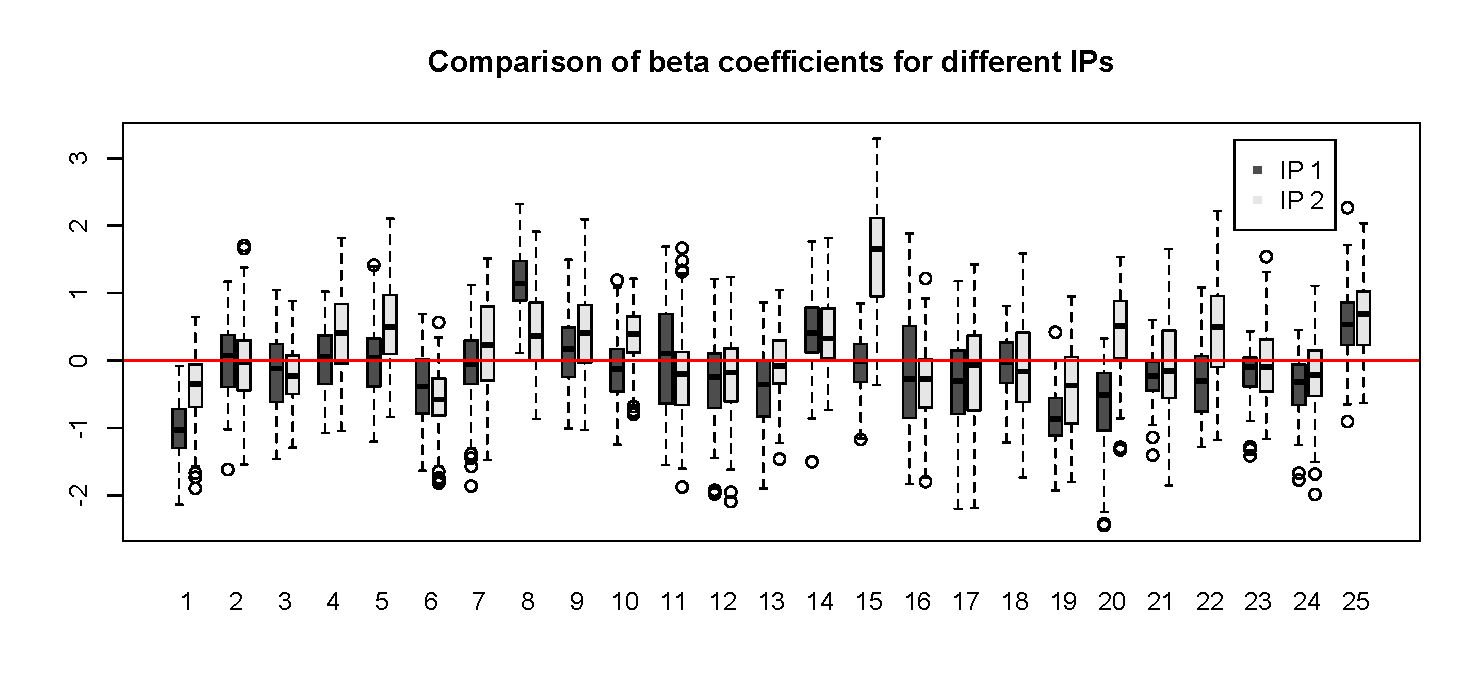
\includegraphics[width=1\textwidth]{betaplot.pdf} 
 	\caption{Posterior distribution of  $\boldsymbol{b}^{(c)}$ for Vance county emails}
 	\label{fig:Vanceboxplot}
 \end{figure}
 \begin{table}[ht]
 	\centering
 	\begin{tabular}{|l|l|l|l|l|l|l|l|l|l|}
 		\hline
 		covariate & 1&2 - 4&5 - 7& 8 - 10 & 11 - 13 & 14 - 16& 17 - 19 & 20 - 22&23 - 25\\
 	\hline	name & intercept & outdegree & indegree & send & receive & 2-send & 2-receive & sibling & cosibling\\
 	 		\hline
 	\end{tabular}
 	\caption {Network statistics}
 \end{table}
 \normalsize
By examining the estimates in Figure 2 and their corresponding interpretation, it seems that there exist strong effects of dynamic network covariates. That is, whether the sender and receiver previously had dyadic or triangle interaction strongly increase the rate of their interactions. \textcolor{red}{What are the findings here?}\newpage
 \begin{figure}[ht]
 	\centering
 		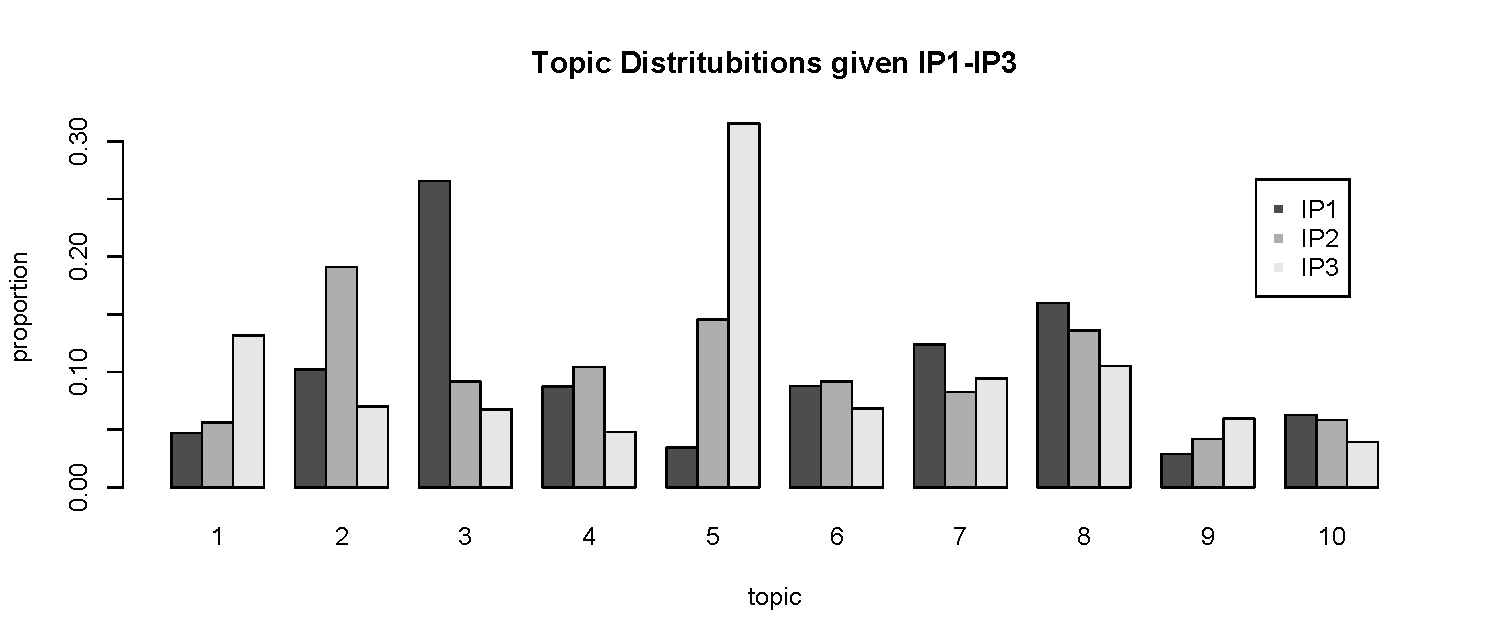
\includegraphics[width=0.7\textwidth]{topicplot.pdf} 
 	\caption{Posterior distribution of $\mathcal{Z}$ for Vance county emails}
 	\label{fig:Vancebarplot}
 \end{figure} 
\noindent Next, we scrutinize the topic distributions in Figure 3. There is some distinctive differences in the topic distributions $\mathcal{Z}$, given the assignment of interaction patterns to the documents $\mathcal{C}$. Specifically, each interaction pattern has different topics as the topic with highest probability.
 \normalsize
 \newline
 Furthermore, we look at the distribution of words given the topics, which corresponds to Algorithm 4 in the generative process. Since the topic-word distribution $\phi$ does not depend on the interaction patterns as previous cases, Table 3 lists top 10 topics with top 10 words that have the highest probability conditioned on the topic. In addition, this time we try to check the interaction pattern-word distribution by listing top 10 words that have the highest probability conditioned on the interaction pattern. It seems that the words are not significantly different, having several words like `director', `phones', `department', `description', or `henderson' (county seat of Vance county) appeared repetitively across the most of the topics or interaction patterns. The word 'will' was ranked the top in most of the lists, probably because it was not deleted during the text mining process while other similar type of words like `am', `is', `are', or `can' are all removed. \\
 \begin{table}[ht]
 	\centering
 	\begin{tabular}{|l||l||}
 		\hline
 		{\textbf{IP1} }&{\textbf{IP2} }\\
 		\hline\hline
 		K=5, K=2 & K=3, K=4, K=1\\
 		\hline
 	operations, description&emergency, electronic, will\\
 	emergency, phase & operations, message, meeting\\
 	henderson, planning& fax, request, director\\
 	director, development & henderson, review, phone\\
 	street, director & street, response, october\\
 	church, henderson& center, records, extension\\
 	suite, fax & director, manager, phones\\
 	office, church & church, pursuant, latest\\ 
 	center, phone & office, ncgs, directory\\
 	communications, email & communications, chapter, attached\\
 		\hline
 	\end{tabular}
 	\caption {Summary of top 10 words that have the highest probability conditioned on the topic}
 	\label{table:VancewordsMCMC}
 \end{table}
 \subsection{Dare county email data} \label{subsec: Dare county email data}
 Dare county data contains $D=2247$ emails between $A=27$ actors, including $W=2907$ vocabulary in total. Again, we used $K=10$ topics and $C=3$ interaction patterns. MCMC sampling was implemented based on the order and scheme illustrated earlier. We set the outer iteration number as $I=1000$, and inner iteration numbers as $n_1=3, n_2=3,$ and $n_3=3300$. In addition, after some experimentation, $\delta_B$ was set as 0.02, to ensure sufficient acceptance rate. In our case, the average acceptance rate for $\boldsymbol{b}$ was 0.277. As demonstrated in Algorithm 5, the last value of $\mathcal{C}$, the last value of $\mathcal{Z}$, and the last $n_3$ length chain of $\mathcal{B}$ were taken as the final posterior samples. Among the $\mathcal{B}$ samples, 300 were discarded as a burn-in and every $10^{th}$ samples were taken. After these post-processing, MCMC diagnostic plots are attached in APPENDIX D, as well as geweke test statistics. 
\bibliographystyle{apalike}
\bibliography{IPTM}
\clearpage
 \section*{APPENDIX}
 \subsection*{APPENDIX A: Notations in IPTM}
  \begin{table}[ht]
  	\centering
  	\scalebox{0.9}{ 	\begin{tabular}{ |c|c|c|} 
  			\hline
  			\hline
  			  			Sender of the $d^{th}$ document&$i^{(d)}$ & Scalar\\
  			  			\hline 
  	  			Receivers of the $d^{th}$ document&$J^{(d)}$ & $|J^{(d)}|$-dimensional vector\\
  	  			\hline 
  	  			Individual receiver of the $d^{th}$ document&$j^{(d)}$ & Scalar\\
  	  			\hline
  			  Time of the $d^{th}$ document&$t^{(d)}$ & Scalar\\
  			  			\hline 			
  			Authors of the corpus &$\mathcal{A}$ & Set\\
  			\hline
  			Number of authors &$A$ & Scalar \\
  			\hline
  			Number of documents &$D$ & Scalar \\
  			\hline
  			Number of words in the $d^{th}$ document &$N^{(d)}$ & Scalar \\
  			\hline
  			Number of topics & $K$ & Scalar \\
  			\hline
  			Vocabulary size & $W$ & Scalar \\
  			\hline
  			Number of interaction patterns &$C$ & Scalar \\
  			\hline
  			Number of words assigned to word and topic&$N^{WK}$ & Scalar \\
  			\hline
  			Interaction pattern of the $k^{th}$ topic&$C_k$ & Scalar\\
  			\hline 
  			Tuning parameter in tie generative process& $\delta$ & Scalar\\
  			\hline 
  			Poisson parameter for number of words $N^{(d)}$& $\zeta$ & Scalar\\ \hline
  			Words in the $d^{th}$ document&$\boldsymbol{w}^{(d)}$ & $N^{(d)}$-dimensional vector\\
  			\hline 
  			$n^{th}$ word in the $d^{th}$ document&${w}_n^{(d)}$ & $n^{th}$  component of $\boldsymbol{w}^{(d)}$\\
  			\hline 	
  			Topic assignments in the $d^{th}$ document&$\boldsymbol{z}^{(d)}$ & $N^{(d)}$-dimensional vector\\
  			\hline 
  			Topic assignments for $n^{th}$ word in the $d^{th}$ document&${z}_n^{(d)}$ & $n^{th}$ component of $\boldsymbol{z}^{(d)}$\\
  			\hline 	
  			Dirichlet concentration prior for document topic distribution&$\alpha$ & Scalar \\
  			\hline	
  			Dirichlet base prior for document topic distribution&$\boldsymbol{m}$ & $K$-dimensional vector \\
  			\hline			
  			Dirichlet concentration prior for topic word distribution&$\beta$ & Scalar \\
  			\hline			 
  			Dirichlet base prior for topic word distribution&$\boldsymbol{u}$ & $W$-dimensional vector  \\
  			\hline				 	
  			Variance of Normal prior&$\sigma^2$ & Scalar \\
  			\hline		
  			Probabilities of the words given topic $k$ &$\boldsymbol{\phi}^{(k)}$ & $W$-dimensional vector\\
  			\hline
  			Probabilities of the topics given the $d^{th}$ document &$\boldsymbol{\theta}^{(d)}$ & $K$-dimensional vector\\
  			\hline		
  			Coefficient of the intensity process given interaction pattern $c$ &$\boldsymbol{b}^{(c)}$ & $p$-dimensional vector\\
  			\hline		
  			Network statistics for $(i, j)$ at time $t$ given interaction pattern $c$ &$\boldsymbol{x}^{(c)}_t{(i,j)}$ & $p$-dimensional vector\\
  			\hline		
  			Stochastic intensity of document $d$ at time $t$ & $\boldsymbol{\lambda}^{(d)}(t)$ & $A\times A$ matrix\\
  			\hline
  		  	Stochastic intensity of $(i, j)$ in document $d$ at time $t$ & ${\lambda}_{ij}^{(d)}(t)$ & Scalar\\
  		  	\hline	
  		  	  		  	Proportion of topics in document $d$ corresponding to interaction pattern $c$ & $p_c^{(d)}$ & Scalar\\
  		  	  		  	\hline
  		  Time increments associated to $(i, J)$ pair & $\Delta T_{iJ}$ & Scalar\\
  		  		\hline
  			\hline
  		\end{tabular}}
  		\caption {Symbols associated with IPTM, as used in this paper}
  		\label{table:SymbolsIPTM}
  	\end{table}
  	\normalsize
  \subsection*{APPENDIX B: Integrating out $\Phi$ and $\Theta$ in latent Dirichlet allocation}
  \begin{equation}
  \begin{aligned}
   &  P(\Phi, \Theta, \mathcal{Z}, \mathcal{C}, \mathcal{B}, \mathcal{W}, \mathcal{I}_{\mbox{a}}, \mathcal{J}_{\mbox{a}}, \mathcal{T}_{\mbox{a}}, \mathcal{I}_{\mbox{o}}, \mathcal{J}_{\mbox{o}}, \mathcal{T}_{\mbox{o}}| \beta, \boldsymbol{u}, \alpha, \boldsymbol{m}, \sigma^2, \delta) \\& 
   \propto P( \mathcal{Z}, \mathcal{C}, \mathcal{B},  \mathcal{W},\mathcal{I}_{\mbox{a}}, \mathcal{J}_{\mbox{a}}, \mathcal{T}_{\mbox{a}}, \mathcal{I}_{\mbox{o}}, \mathcal{J}_{\mbox{o}}, \mathcal{T}_{\mbox{o}}|\Phi, \Theta, \sigma^2, \delta)P(\Phi, \Theta| \beta, \boldsymbol{u}, \alpha, \boldsymbol{m})
   \\& 
 \propto P(\mathcal{Z}|\mathcal{W},\Theta)P(\mathcal{C})P(\mathcal{B}|\mathcal{C}, \sigma^2)P(\mathcal{W}|\Phi)P(\Phi| \beta, \boldsymbol{u})P(\Theta|\alpha, \boldsymbol{m})P(\mathcal{I}_{\mbox{a}}, \mathcal{J}_{\mbox{a}}, \mathcal{T}_{\mbox{a}},\mathcal{I}_{\mbox{o}}, \mathcal{J}_{\mbox{o}}, \mathcal{T}_{\mbox{o}} |\mathcal{Z}, \mathcal{C}, \mathcal{B}, \delta)
  \\&=\Big[\prod_{d=1}^{D}\prod_{n=1}^{N^{(d)}} P( z_n^{(d)}|w_n^{(d)},  \boldsymbol{\theta}^{(d)})\Big]\times \Big[\prod_{k=1}^{K} P(C_k)\Big] \times\Big[\prod_{c=1}^{C} P( \boldsymbol{b}^{(c)}| \sigma^2)\Big] \times\Big[\prod_{d=1}^{D}\prod_{n=1}^{N^{(d)}} P(w_n^{(d)}| \phi_{z_n^{(d)}})\Big]\times \Big[\prod_{k=1}^{K} P( \boldsymbol{\phi}^{(k)}| \beta, \boldsymbol{u})\Big]\\&\quad \quad\times \Big[\prod_{d=1}^{D} P( \boldsymbol{\theta}^{(d)}|\alpha, \boldsymbol{m})\Big]\times\Big[\prod_{d=1}^{D} P(\mathcal{I}^{(d)}_{\mbox{a}}, \mathcal{J}^{(d)}_{\mbox{a}}, \mathcal{T}^{(d)}_{\mbox{a}}, i^{(d)}_{\mbox{o}}, J^{(d)}_{\mbox{o}}, t^{(d)}_{\mbox{o}} |\mathcal{I}^{(<d)}_{\mbox{o}}, \mathcal{J}^{(<d)}_{\mbox{o}}, \mathcal{T}^{(<d)}_{\mbox{o}},\mathcal{Z}, \mathcal{C}, \mathcal{B}, \delta)\Big] 
  \end{aligned}
  \end{equation}
  Dropping the terms independent of tokens out, we further rewrite the equation (28) as below:
  \begin{equation}
  \begin{aligned}
  & \propto \Big[\prod_{d=1}^{D}\prod_{n=1}^{N^{(d)}} P(z_n^{(d)}|w_n^{(d)},  \boldsymbol{\theta}^{(d)})\Big]\times\Big[\prod_{d=1}^{D}\prod_{n=1}^{N^{(d)}} P(w_n^{(d)}| \phi_{z_n^{(d)}})\Big]\times \Big[\prod_{k=1}^{K} P( \boldsymbol{\phi}^{(k)}| \beta, \boldsymbol{u})\Big] \times\Big[\prod_{d=1}^{D} P( \boldsymbol{\theta}^{(d)}|\alpha, \boldsymbol{m})\Big] \\&
  \propto\Big[\prod_{d=1}^{D}\prod_{n=1}^{N^{(d)}} \phi_{w_n^{(d)}z_n^{(d)}}\Big]\times \Big[\prod_{d=1}^{D}\prod_{n=1}^{N^{(d)}} \boldsymbol{\theta}^{(d)}_{z_n^{(d)}}\Big]\\&\quad\quad \times \Big[\prod_{k=1}^{K} \Big(\frac{\Gamma(\sum_{w=1}^{W}\beta u_w)}{\prod_{w=1}^{W}\Gamma(\beta u_w)}\prod_{w=1}^{W}\phi_{wk}^{\beta u_w-1} \Big)\Big]\times \Big[\prod_{d=1}^{D} \Big(\frac{\Gamma(\sum_{k=1}^{K}\alpha m_k)}{\prod_{k=1}^{K}\Gamma(\alpha m_k)}\prod_{k=1}^{K}(\boldsymbol{\theta}^{(d)}_{k})^{\alpha m_k-1} \Big)\Big] \\&
  \propto\Big[\frac{\Gamma(\sum_{w=1}^{W}\beta u_w)}{\prod_{w=1}^{W}\Gamma(\beta u_w)}\Big]^K \times \prod_{d=1}^{D} \Big[\frac{\Gamma(\sum_{k=1}^{K}\alpha m_k)}{\prod_{k=1}^{K}\Gamma(\alpha m_k)}\Big]\times
  \Big[\prod_{k=1}^{K}\prod_{w=1}^{W}\phi_{wk}^{N^{WK}_{wk}+\beta u_w-1}\Big]\times\Big[\prod_{d=1}^{D}\prod_{k=1}^{K}(\boldsymbol{\theta}^{(d)}_{k})^{N_{k|d}+\alpha m_k-1}\Big]
  \end{aligned}
  \end{equation}
  where $N^{WK}_{wk}$ is the number of times the $w^{th}$ word in the vocabulary is assigned to topic $k$, and $N_{k|d}$ is the number of times topic k shows up in the document $d$. By looking at the forms of the terms involving  $\Theta$ and $\Phi$ in Equation (21), we integrate out the random variables $\Theta$ and $\Phi$, making use of the fact that the Dirichlet distribution is a conjugate prior of multinomial distribution. Applying the well-known formula $\int\prod_{n=1}^{M}[x_m^{k_m-1}dx_m]=\frac{\prod_{n=1}^M\Gamma(k_m)}{\Gamma(\sum_{n=1}^Mk_m)}$ to (22), we have:
  \begin{equation}
  \begin{aligned}
  &P(\mathcal{Z}, \mathcal{C}, \mathcal{B}, \mathcal{W}, \mathcal{I}_{\mbox{a}}, \mathcal{J}_{\mbox{a}}, \mathcal{T}_{\mbox{a}}, \mathcal{I}_{\mbox{o}}, \mathcal{J}_{\mbox{o}}, \mathcal{T}_{\mbox{o}}| \beta, \boldsymbol{u}, \alpha, \boldsymbol{m}, \sigma^2,  \delta)\\&=\mbox{Const.}\int_{\Theta}\int_{\Phi}\Big[\prod_{k=1}^{K}\prod_{w=1}^{W}\phi_{wk}^{N^{WK}_{wk}+\beta u_w-1}\Big]\Big[\prod_{d=1}^{D}\prod_{k=1}^{K}(\boldsymbol{\theta}^{(d)}_{k})^{N_{k|d}+\alpha m_k-1}\Big]d\Phi d\Theta
  \\&=\mbox{Const.}\Big[\prod_{k=1}^{K}\int_{\phi_{:k}}\prod_{w=1}^{W}\phi_{wk}^{N^{WK}_{wk}+\beta u_w-1  }d\phi_{:k}\Big]\times\Big[\prod_{d=1}^{D}\int_{\theta_{:d}}\prod_{k=1}^{K}(\boldsymbol{\theta}^{(d)}_{k})^{N_{k|d}+\alpha m_k-1}d\theta_{:d}\Big]
  \\&=\mbox{Const.}\Big[\prod_{k=1}^{K}\frac{\prod_{w=1}^W\Gamma(N_{wk}^{WK}+\frac{\beta}{W})}{\Gamma(\sum_{w=1}^WN_{wk}^{WK}+\beta )}\Big]\times\Big[\prod_{d=1}^{D}\frac{\prod_{k=1}^K\Gamma(N_{k|d}+\alpha m_k)}{\Gamma(N_{\cdot|d}+\alpha)}\Big].
  \end{aligned}
  \end{equation}
  \subsection*{APPENDIX C: Conditional probability of $\mathcal{Z}$}
  \begin{equation}
  \begin{aligned}
  & P(\boldsymbol{w}^{(d)}, \boldsymbol{z}^{(d)}|\mathcal{W}_{\backslash d}, \mathcal{Z}_{\backslash d}, \beta, \boldsymbol{u}, \alpha, \boldsymbol{m}) \\& \propto \prod_{n=1}^{N^{(d)}}P(z^{(d)}_n=k, w^{(d)}_n=w| \mathcal{W}_{\backslash d, n}, \mathcal{Z}_{\backslash d, n}, \beta, \boldsymbol{u}, \alpha, \boldsymbol{m})
  \end{aligned}
  \end{equation} 
  To obtain the Gibbs sampling equation, we need to obtain an expression for $P(z^{(d)}_n=k,  w^{(d)}_n=w|\mathcal{W}_{\backslash d, n}, \mathcal{Z}_{\backslash d, n}, \beta, \boldsymbol{u}, \alpha, \boldsymbol{m})$,
  From Bayes' theorem and Gamma identity $\Gamma(k+1)=k\Gamma(k)$,
  \begin{equation}
  \begin{aligned}
  & P(z^{(d)}_n=k, w^{(d)}_n=w|\mathcal{W}_{\backslash d, n}, \mathcal{Z}_{\backslash d, n}, \beta, \boldsymbol{u}, \alpha, \boldsymbol{m}) \\& \propto 
  \frac{P(\mathcal{W}, \mathcal{Z}|\beta, \boldsymbol{u}, \alpha, \boldsymbol{m})}{P(\mathcal{W}_{\backslash d, n}, \mathcal{Z}_{\backslash d, n}|\beta, \boldsymbol{u}, \alpha, \boldsymbol{m})}\\& \propto \frac{\prod_{k=1}^{K}\frac{\prod_{w=1}^W\Gamma(N_{wk}^{WK}+\beta u_w)}{\Gamma(\sum_{w=1}^WN_{wk}^{WK}+\beta )}\times\prod_{k=1}^K\frac{\Gamma(N_{k|d}+\alpha m_k)}{\Gamma(N_{\cdot|d}+\alpha)}}{\prod_{k=1}^{K}\frac{\prod_{w=1}^W\Gamma(N_{wk, \backslash d, n}^{WK}+\beta u_w)}{\Gamma(\sum_{w=1}^WN_{wk, \backslash d, n}^{WK}+\beta )}\times\prod_{k=1}^K\frac{\Gamma(N_{k|d, \backslash d, n}+\alpha m_k)}{\Gamma(N_{\cdot|d, \backslash d, n}+\alpha)}}\\ & \propto 
  \frac{N_{wk, \backslash d, n}^{WK}+\frac{\beta}{W}}{\sum_{w=1}^WN_{wk,  \backslash d, n}^{WK}+\beta}\times\frac{N_{k|d, \backslash d, n}+\alpha m_k}{N^{(d)}-1+\alpha}
  \end{aligned}
  \end{equation}
  Then, same as for LDA, we also know that the topic assignment $z_n^{(d)}=k$ is obtained by:
  \begin{equation}
  \begin{aligned}
  &P(z^{(d)}_n=k|w^{(d)}_n=w, \mathcal{W}_{\backslash d, n}, \mathcal{Z}_{\backslash d,n}, \beta, \boldsymbol{u}, \alpha, \boldsymbol{m}) \propto
  \frac{N_{k|d, \backslash d, n}+\alpha m_k}{N^{(d)}-1+\alpha}
  \end{aligned}
  \end{equation}
  In addition, the conditional probability that a new word generated in the document would be $w_n^{(d)}=w$, given that it is generated from topic $z_n^{(d)}=k$ is obtained by:
  \begin{equation}
  \begin{aligned}
  & P(w^{(d)}_m=w|z^{(d)}_m=k, \mathcal{W}_{\backslash d, n}, \mathcal{Z}_{\backslash d, nm}, \beta, \boldsymbol{u}, \alpha, \boldsymbol{m}) \propto 
  \frac{N_{wk, \backslash d, n}^{WK}+\frac{\beta}{W}}{\sum_{w=1}^WN_{wk, \backslash d, n}^{WK}+\beta}
  \end{aligned} 
  \end{equation}
  NOTE: Using Equation (28), the unnormalized constant we use to check the model convergence and the corresponding log-constant is,
  \begin{equation}
  \begin{aligned}
  & \prod_{d=1}^{D}\prod_{n=1}^{N^{(d)}}  P(z^{(d)}_n=k, w^{(d)}_n=w|\mathcal{W}_{\backslash d, n}, \mathcal{Z}_{\backslash d,m}, \beta, \boldsymbol{u}, \alpha, \boldsymbol{m}) \\ & \propto \prod_{d=1}^{D}\prod_{n=1}^{N^{(d)}} 
  \frac{N_{w^{(d)}_nz^{(d)}_n, \backslash d, n}^{WK}+\frac{\beta}{W}}{\sum_{w=1}^WN_{wz^{(d)}_n,  \backslash d, n}^{WK}+\beta}\times\frac{N_{k|d, \backslash d, n}+\alpha m_{z^{(d)}_n}}{N^{(d)}-1+\alpha},
  \end{aligned}
  \end{equation}
  \begin{equation}
  \begin{aligned}
  & \sum_{d=1}^{D}\sum_{n=1}^{N^{(d)}} \mbox{log}\Big( P(z^{(d)}_n=k, w^{(d)}_n=w|\mathcal{W}_{\backslash d, n}, \mathcal{Z}_{\backslash d, n}, \beta, \boldsymbol{u}, \alpha, \boldsymbol{m})\Big) \\ & \propto \sum_{d=1}^{D}\sum_{n=1}^{N^{(d)}} 
  \mbox{log}\Big(N_{w^{(d)}_mz^{(d)}_m, \backslash d, n}^{WK}+\frac{\beta}{W}\Big)-\mbox{log}\Big(\sum_{w=1}^WN_{wz^{(d)}_m,  \backslash d, n}^{WK}+\beta\Big)\\&+\mbox{log}\Big(N_{k|d, \backslash d, n}+\alpha m_{z^{(d)}_m}\Big)-\mbox{log}\Big(N^{(d)}-1+\alpha\Big)
  \end{aligned}
  \end{equation}
  \subsection*{APPENDIX D: More results on Vance county}
 \begin{figure}[ht]
 	\centering
 	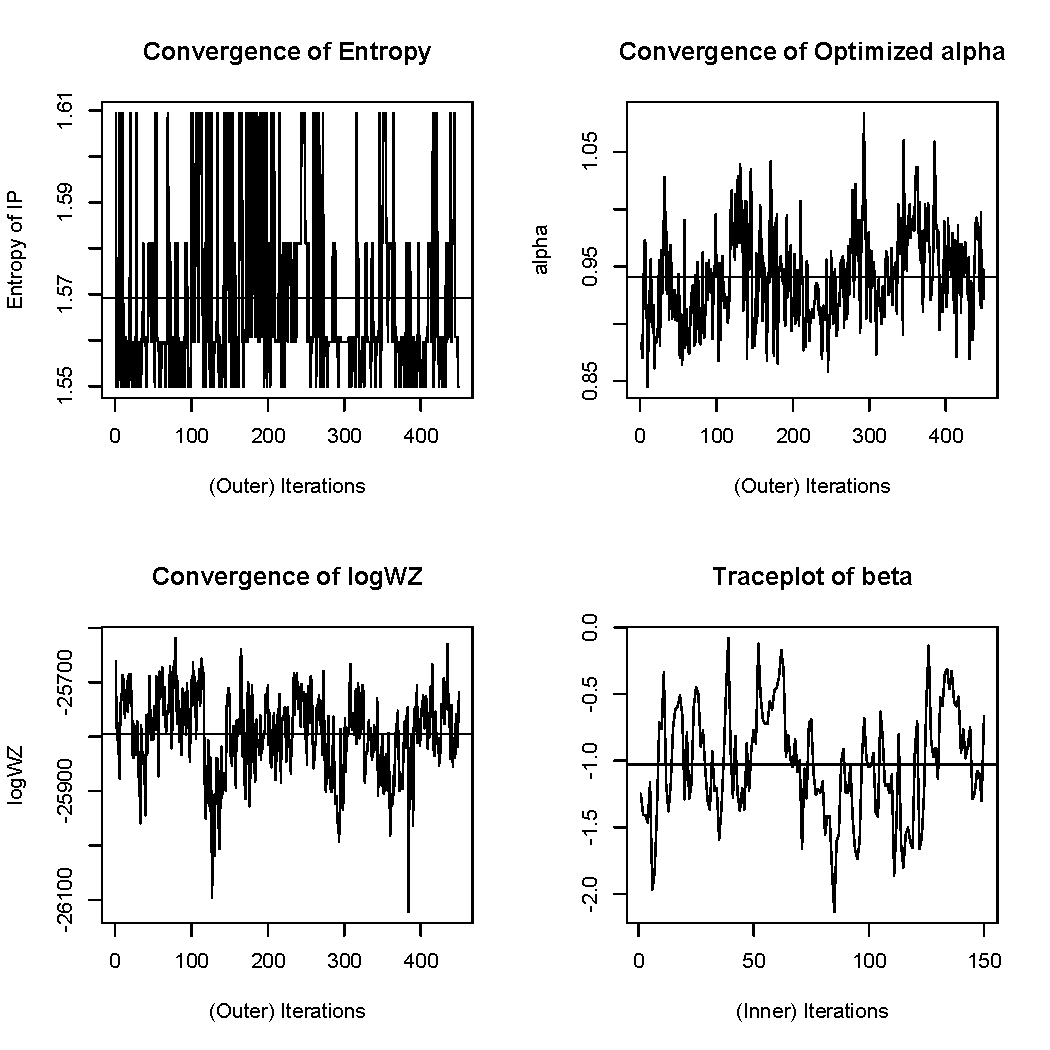
\includegraphics[width=0.7\textwidth]{convergence500.pdf} 
 	\caption{Convergence plot}
 	\label{fig:Convergence plot}
 \end{figure}
  \subsection*{APPENDIX E: Getting It Right}
\subsubsection*{Backward Generative Process} \label{subsubsec: Backward Generative Process}
We need to define a “backward” generative process in order to perform Geweke’s “Getting it Right” test because when we are generating our “backwards” samples, we only want to resample the token word types and (sender, recipients, timestamp) pairs, and not any of
our latent variables. This means we will take as input the latent variables we got by running our inference procedure (token topic assignments, topic interaction pattern assignments, and interaction pattern parameters), and simply condition on these to draw new data.
This “backward” version of the generative process is detailed below.\\ \newline
Let $NKV$ be a $V\times K$ dimensional matrix where each entry will record the count of the number of tokens of word-type $v$ that are currently assigned to topic $k$. Also let $NK$ be a $K$ dimensional vector recording the total count of tokens currently assigned to topic $k$. These
data structures, along with the latent variables we got by running our inference procedure (token topic assignments, topic interaction pattern assignments, interaction pattern parameters, and tuning parameter $\delta$) are passed in to the backward generative process, which then outputs new documents with the generated token word types and (sender, recipients, timestamp) pairs.
\begin{algorithm}[H]
	\SetAlgoLined
	\caption{Generate data with backward sampling}
	\For{d=1 to D}{
		set $N^{(d)}= \mbox{max}(1, \bar N^{(d)})$, where $\bar N^{(d)}$ is known\\
		\For{n=1 to ${N}^{(d)}$}{
			\If {$\bar N^{(d)}>0$} {
				$NKV_{v_n, k_n} -=1$\\
				\For{v=1 to $V$}{
				 $\phi_n^{(d)}[v] = \frac{NKV_{v, z_n^{(d)}}+\beta\boldsymbol{u}}{NK_k + \beta}$
					}
				draw $w_n^{(d)} \sim \phi_n^{(d)}$\\
				$NKV_{w_n^{(d)}, z_n^{(d)}} += 1$
			}
	}
	              \For{i=1 to $A$}{
	              	\For{j=1 to $A$}{
	              		\If {j $\neq$ i} {
	              			calculate $\boldsymbol{x}_{t_+^{(d-1)}}^{(c)}(i, j)$, the network statisitcs evaluated at time $t_+^{(d-1)}$  \\
	              			set $\lambda^{(d)}_{ij}=\sum\limits_{c=1}^{C} p^{(d)}_c\cdot\mbox{exp}\Big\{\boldsymbol{b}^{(c)T}\boldsymbol{x}^{(c)}_{t^{(d-1)}_+}(i, j)\Big\}\cdot 1\{j \in \mathcal{A}_{\backslash i}\}$\\
	              			draw I($i \rightarrow j$) $\sim \mbox{Ber}(\frac{\delta\lambda^{(d)}_{ij}}{\delta\lambda^{(d)}_{ij}+1})$}  }
	              	draw $\Delta T_{iJ_i} \sim \mbox{Exp}(\lambda_{iJ_i}^{(d)})$
	              }
	              set $t^{(d)} = t^{(d-1)}+\mbox{min}(\Delta T_{i{J_i}})$, $i^{(d)} = i_{\mbox{min}(\Delta T_{i{J_i}})}$, and $J^{(d)} = J_{i^{(d)}}$
	              
		}
\end{algorithm}
\end{document}

